\chapter{Asynchronous Programming}

Now a days, providing a modest experience on a mobile app, or even rendering
simple web pages typically requires the collaboration of dozens of network
services each speaking many different languages or protocols to one another.
Such systems are one of many flavors of a {\em distributed system}, and as such
must coordinate between many network requests to, as quickly and reliably as
possible, piece together an interface or some other user experience.

Responsiveness is a requirement. Yet providing a responsive experience is at
odds with the need to piece together the results from many calls over the
network to other services. Synchronously making a request to a remote service
and blocking, or waiting, until that request is fulfilled before moving on to
the next request is slow -- roundtrip network communication is known to be
1,000,000 to 10,000,000 times slower than roundtrips to main
memory~\cite{LatencyNumbersEveryProgrammerShouldKnow} -- and making requests
sequentially, one by one, is also often unnecessary.

Asynchronous programming solves these problems by separating the execution of
individual tasks (\eg calls to network services) from the main program flow. In
a language like Scala where tasks can be executed by multiple threads, this
reduces blocking because rather than stopping a thread to wait on the completion
of another task, a separate task is simply scheduled to proceed when the
resource its waiting for becomes available. Thus freeing up the thread that
would otherwise be waiting to do more meaningful work.
% That is, Unlike conventional parallelism, asynchronous parallelism

In this chapter, we will see two abstractions for fully non-blocking,
asynchronous programming; functionally-inspired {\em futures and promises} in
Scala~\cite{Futures} in Section~\ref{sec:futures} and a generalization of
futures to a pool or multiset-type data structure called {\em
FlowPools}~\cite{FlowPools} in Section~\ref{sec:flowpools}.

% \section{Motivation}
%
% Asynchronous computation, \eg managing requests.
%
% Multicore architectures have become ubiquitous-- even most mobile devices now
% ship with multiple core processors. Yet parallel programming has yet to enter
% the daily workflow of the mainstream developer. One significant obstacle is an
% undesirable choice programmers must often face when solving a problem that
% could greatly benefit from leveraging available parallelism. Either choose a
% non-deterministic, but performant, data structure or programming model, or
% sacrifice performance for the sake of clarity and correctness.
%
% Programming models based on \emph{dataflow} \cite{Arvind89,CnC10} have the
% potential to simplify parallel programming, since the resulting programs are
% deterministic. Moreover, dataflow programs can be expressed more declaratively
% than programs based on mainstream concurrency constructs, such as shared-memory
% threads and locks, as programmers are only required to specify data and
% control dependencies. This allows one to reason sequentially about the
% intended behavior of their program, meanwhile enabling the underlying
% framework to effectively extract parallelism.

\section{Futures}
\label{sec:futures}

{\em Futures and promises} can be thought of as, together, a unified abstraction
used for synchronization in programming languages with support for concurrency.
Futures and promises in Scala~\cite{Futures} stand out from their Java
counterparts in two ways; (a) they are functionally-inspired with monadic
combinators and are thus composable, and (b) they are fully asynchronous and
non-blocking by default. A visualization of this blocking difference and
definition is shown in Figures~\ref{fig:future-promise-blocking}
and~\ref{fig:future-promise-async}. Here, the central green arrow in each figure
can be thougth of as the main program thread.

\begin{figure}[!t]
\centering
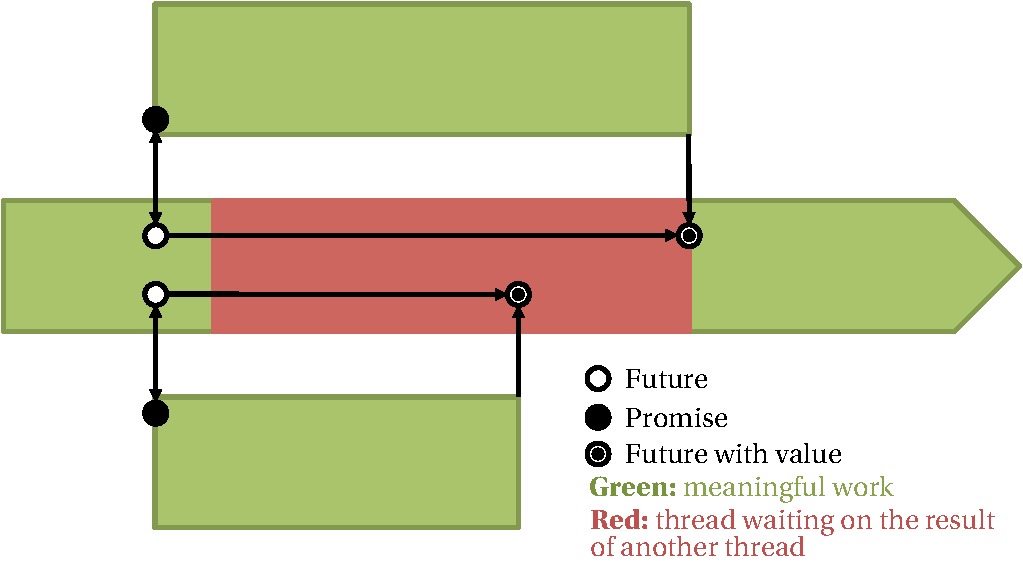
\includegraphics[width=0.75\textwidth]{images/future-promise-basic-async-blocking}
% \setlength{\abovecaptionskip}{-10pt}
% \setlength{\belowcaptionskip}{-20pt}
\caption{Illustration of blocking futures, as in Java. The central green arrow can be thought of as the main program thread.}
\label{fig:future-promise-blocking}
\end{figure}

\begin{figure}[!t]
\centering
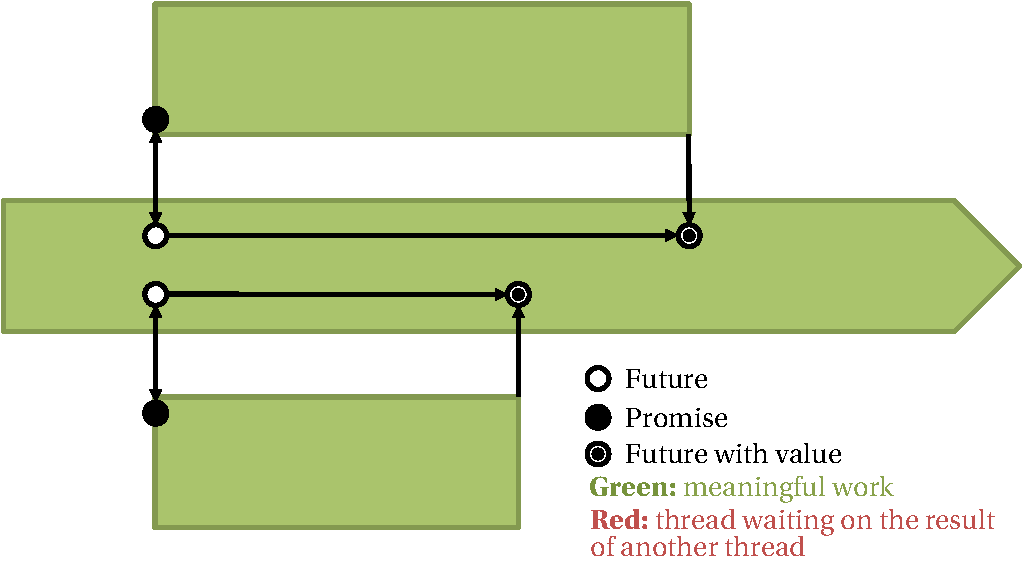
\includegraphics[width=0.75\textwidth]{images/future-promise-basic-async}
% \setlength{\abovecaptionskip}{-10pt}
% \setlength{\belowcaptionskip}{-20pt}
\caption{Illustration of fully asynchronous, non-blocking futures, as in Scala. The central green arrow can be thought of as the main program thread.}
\label{fig:future-promise-async}
\end{figure}


A {\em future} can be thought of as a container which represents a value that
will eventually be computed. They're related to {\em promises} in that a future
is a read-only window to a single-assignment (write-once) variable called a {\em
promise}. This relationship is illustrated in
Figure~\ref{fig:future-promise-basic}.

\begin{figure}[!t]
\centering
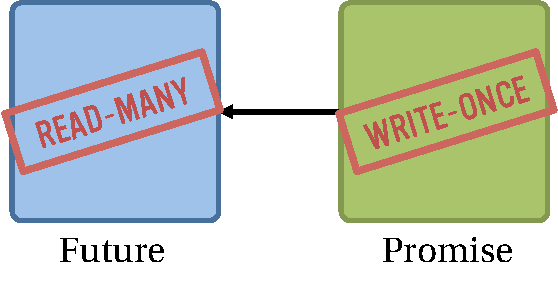
\includegraphics[width=0.5\textwidth]{images/future-promise-basic}
% \setlength{\abovecaptionskip}{-10pt}
% \setlength{\belowcaptionskip}{-20pt}
\caption{Futures and promises can be thought of as a single concurrency abstraction.}
\label{fig:future-promise-basic}
\end{figure}

Before a future's result is computed, we say that the future is {\em not
completed}. If the computation representing a future is finished with a value or
an exception, we say that the future is {\em completed}. Completion can take one
of two forms: (a) when a future is completed with a value, we say the future was
{\em successfully completed} with that value, or (b) when a future is completed
with an exception thrown by the computation, we say the future was {\em failed}
with that exception.

\subsection{Basic Usage}

The type of \verb|Future| and \verb|Promise| is as follows: ({\em simplified})

% \begin{minipage}[t]{0.4\linewidth}
% % \begin{minted}{scala}
% % trait Future[T] {
% %   def onSuccess(f: T => Unit): Unit
% % }
% % \end{minted}
% \begin{minipage}[t]{0.4\linewidth}
% % \begin{minted}{scala}
% % trait Promise[T] {
% %   def success(elem: T): Unit
% %   def future: Future[T]
% % }
% % \end{minted}
% \end{minipage}

\begin{minipage}[t]{0.5\linewidth}
\begin{minted}{scala}
trait Future[T] {
  def onSuccess(f: T => Unit): Unit
}
\end{minted}
\end{minipage}
\begin{minipage}[t]{0.5\linewidth}
\begin{minted}{scala}
trait Promise[T] {
  def success(elem: T): Unit
  def future[T]: Future[T]
}
\end{minted}
\end{minipage}

As depicted visually in Figure~\ref{fig:future-promise-basic}, every
\verb|Promise[T]| can return a reference to its corresponding \verb|Future| with
the \verb|future| method.

An example of how a future can be created is as follows. Let’s assume that we
want to use a hypothetical API of some popular social network to obtain a list
of friends for a given user. We will open a new session and then send a request
to obtain a list of friends of a particular user:

\begin{minted}{scala}
val session = ... // obtain a list of friends for some user/credentials
val f: Future[List[Friend]] = Future {
  session.getFriends() // network call to get a list of that user's friends
}
\end{minted}

To obtain the list of friends of a user, a request has to be sent over a
network, which can take a long time. This is illustrated with the call to the
method \verb|getFriends| that returns \verb|List[Friend]|. To better utilize the
CPU until the response arrives, we should not block the rest of the program --
this computation should be scheduled asynchronously. The future method does
exactly that--it performs the specified computation block concurrently, in this
case sending a request to the server and waiting for a response.

The list of friends becomes available in the future \verb|f| once the server
responds.

An unsuccessful attempt may result in an exception. In the following example,
the session value is incorrectly initialized, so the computation in the future
block will throw a \verb|NullPointerException|. This future \verb|f| is then
failed with this exception instead of being completed successfully:

\begin{minted}{scala}
val session = null
val f: Future[List[Friend]] = Future {
  session.getFriends
}
\end{minted}

We now know how to start an asynchronous computation to create a new future
value, but we have not shown how to use the result once it becomes available, so
that we can do something useful with it. Once created, a future may be used in
one of two ways, either via:

\begin{itemize}
  \itemsep0em
  \item {\em callbacks}, or
  \item {\em composable higer-order combinators}, such as \verb|map|, \verb|flatMap|, and \verb|filter|.
\end{itemize}

We will see how to use both callbacks and higher-order functions to interact
with to-be-computed values in the following two subsections.

\subsection{Callbacks}

One way to interact with the result of a future computation in a non-blocking
way is to attach a callback to perform some side-effecting operation such as
completing another future. Callbacks are a typical way to do asynchronous
computation--a callback is a function that is called once its arguments become
available. There are three methods provided to work with callbacks on Scala's
futures:

\begin{itemize}
  \itemsep0em
  \item \verb|def foreach[U](f: (T) => U): Unit|
  \item \verb|def onComplete[U](f: (Try[T]) => U): Unit|
  \item \verb|def onSuccess[U](pf: PartialFunction[T, U]): Unit|
  \item \verb|def onFailure[U](pf: PartialFunction[Throwable, U]): Unit|
\end{itemize}

The most general form of registering a callback is by using the
\verb|onComplete| method, which takes a callback function of type
\verb|Try[T]=>U| \footnote{\texttt{Try[T]} can be thought of as being similar to
\texttt{Option[T]} or an \texttt{Either[T, S]} in that it is a container type.
However, it has been specifically designed to either hold a value or some
throwable object. \texttt{Try[T]} is a \texttt{Success[T]} when it holds a value
and otherwise \texttt{Failure[T]}, which holds an exception. Another way to
think of \texttt{Try[T]} is to consider it as a special version of
\texttt{Either[Throwable, T]}, specialized for the case when the left value is a
\texttt{Throwable}. }. The callback is applied to the value of type
\verb|Success[T]| if the future completes successfully, or to a value of type
\verb|Failure[T]| otherwise.

To get a feeling for how \verb|onComplete| is used, let's use a running example.
Let's assume for a given social network, we want to fetch a list of our own
recent posts and render them to the screen. We can do this with
\verb|onComplete|:

\begin{minted}{scala}
val f: Future[List[String]] = Future {
  session.getRecentPosts
}
f onComplete {
  case Success(posts) => for (post <- posts) println(post)
  case Failure(t) => println("An error has occured: " + t.getMessage)
}
\end{minted}

The \verb|onComplete| method is general in the sense that it allows the client
to handle the result of both failed and successful future computations. To
handle only successful results, the \verb|onSuccess| callback is used (which
takes a partial function). Similarly, to handle failed results, the
\verb|onFailure| callback is used:

\begin{minted}{scala}
val f: Future[List[String]] = Future {
  session.getRecentPosts
}
f onFailure {
  case t => println("An error has occured: " + t.getMessage)
}
f onSuccess {
  case posts => for (post <- posts) println(post)
}
\end{minted}

The \verb|onComplete|, \verb|onSuccess|, and \verb|onFailure| methods have
result type \verb|Unit|, which means invocations of these methods cannot be
chained. This design is intentional, to avoid suggesting that chained
invocations may imply an ordering on the execution of the registered callbacks
(callbacks registered on the same future are unordered).

% Another way to attach callbacks is via the \verb|foreach| method, which
% asynchronously processes the value in the future once the value becomes
% available. However, it will not be called if the future fails.


\subsection{Higher-Order Combinators}

While callbacks work reasonably well in simple situations, they can quickly get
out of hand and when numerous, they can become difficult to reason about.
Programmers affectoinately refer to this situation as {\em callback hell}.

Scala's futures provide combinators which allow a more straightforward
composition.  What's more, due to the type signature of these methods (they each
return another \verb|Future|), it's possible to {\em compose} operations on
futures and to build up rich computation graphs. The three basic functional
combinators on futures include:

\begin{itemize}
  \itemsep0em
  \item \verb|def map[S](f: (T) => S): Future[S]|
  \item \verb|def flatMap[S](f: (T) => Future[S]): Future[S]|
  \item \verb|def filter(p: (T) => Boolean): Future[T]| {\em (Also, \verb|withFilter|)}
\end{itemize}

To get a feeling for how to use these combinators, and later, how to {\em
pipeline} or {\em chain} them together to build up computation graphs, let's
start with a simple example.

Assume we have an API for interfacing with a currency trading service. Suppose
we want to buy US dollars, but only when it’s profitable. One of the basic
combinators is \verb|map|, which, given a future and a mapping function for the
value of the future, produces a new future that is completed with the mapped
value once the original future is successfully completed. We can use the
\verb|map| combinator to handle the successful case:

\begin{minted}{scala}
val rateQuote = Future {
  connection.getCurrentValue(USD)
}
val purchase = rateQuote map { quote =>
  if (isProfitable(quote)) connection.buy(amount, quote)
  else throw new Exception("not profitable")
}
purchase onSuccess {
  case _ => println("Purchased " + amount + " USD")
}
\end{minted}

Here, we start by creating a future rateQuote which gets the current exchange
rate. After this value is obtained from the server and the future successfully
completed, we call \verb|map| on \verb|rateQuote|, which applies the function
which checks whether or not it's profitable to buy US dollars, and if so, it
buys some amount of the currency. If we now decide to sell some other currency,
it suffices to use map on purchase again.

But what happens if \verb|isProfitable| returns false, hence causing an
exception to be thrown? In this case, \verb|purchase| is failed with that
exception. Furthermore, imagine that the connection was broken and that
\verb|getCurrentValue| threw an exception, failing \verb|rateQuote|. In this
case there would be no value to map, so the purchase would automatically be
failed with the same exception as \verb|rateQuote|.

In conclusion, if the original future is completed successfully then the
returned future is completed with a mapped value from the original future. If
the mapping function throws an exception the future is completed with that
exception. If the original future fails with an exception then the returned
future also contains the same exception. This exception propagating semantics is
present in the rest of the combinators, as well.

Importantly, since the methods \verb|map|, \verb|flatMap|, and \verb|withFilter|
methods are provided on futures (there is an automatic desugaring from
for-comprehensions to calls of these methods), Scala can provide built-in
support for doing using for-comprehensions on futures. We will now see an
example where a for-comprehension is desirable over using chained higher-order
combinators.

In this example, let's assume that we want to exchange US dollars for Swiss
francs (CHF). We have to fetch quotes for both currencies, and then decide on
buying based on both quotes. Here is what this example would look like using for-comprehension syntax:

\begin{minted}{scala}
val usdQuote = Future { connection.getCurrentValue(USD) }
val chfQuote = Future { connection.getCurrentValue(CHF) }
val purchase = for {
  usd <- usdQuote
  chf <- chfQuote
  if isProfitable(usd, chf)
} yield connection.buy(amount, chf)
purchase onSuccess {
  case _ => println("Purchased " + amount + " CHF")
}
\end{minted}

The purchase \verb|future| is completed only once both \verb|usdQuote| and
\verb|chfQuote| are completed--it depends on the values of both these futures so
its own computation cannot begin earlier.

The for-comprehension above is translated into:
\begin{minted}{scala}
val purchase = usdQuote flatMap {
  usd =>
  chfQuote
    .withFilter(chf => isProfitable(usd, chf))
    .map(chf => connection.buy(amount, chf))
}
\end{minted}

Here, the \verb|flatMap| operation maps its own value into some other future.
Once this different future is completed, the resulting future is completed with
its value. In our example, \verb|flatMap| uses the value of the \verb|usdQuote|
future to map the value of the \verb|chfQuote| into a third future which sends a
request to buy a certain amount of Swiss francs. The resulting future
\verb|purchase| is completed only once this third future returned from
\verb|map| completes.

% A fundamental building block of dataflow is the notion of {\em futures and
% promises}.



%
% Dataflow variables in Oz are blocking. Futures in Java are blocking.
%
% Callback-based asynchronous programming.
%
% % \subsection{Promises}
% % \label{sec:promises}
%
% \cite{PromisesLiskov}

% \subsection{\texttt{Try} Type}
% \label{sec:try-type}
%
% \subsection{Functional Composition}
% \label{sec:futures-functional}

\subsection{Exceptions and Recovery}
\label{sec:futures-exceptions}

Futures in Scala also come with a number of combinator methods specialized on
handling failures by providing alternate operations in the event of a failure.
The three main combinators for managing failure are:

\begin{itemize}
  \itemsep0em
  \item \verb|def recover[U >: T](pf: PartialFunction[Throwable, U]): Future[U]|
  \item \verb|def recoverWith[U >: T](pf: PartialFunction[Throwable, Future[U]]): Future[U]|
  \item \verb|def transform[S](s: T => S, f: Throwable => Throwable): Future[S]|
\end{itemize}

To get a feeling for how these work, let's return to the previous example of
purchasing currencies. Let's assume that based on the \verb|rateQuote|
introduced above, we decide to buy a certain amount of some currency. The
\verb|connection.buy| method takes an \verb|amount| to buy and the expected
\verb|quote|. It returns the amount bought. If the quote has changed in the
meantime, it will throw a \verb|QuoteChangedException| and it will not buy
anything. If we want our future to contain 0 instead of the exception, we use
the \verb|recover| combinator:

\begin{minted}{scala}
val purchase: Future[Int] = rateQuote map {
  quote => connection.buy(amount, quote)
} recover {
  case QuoteChangedException() => 0
}
\end{minted}

Here, \verb|recover| combinator creates a new future which holds the same result
as the original future if it completed successfully. If it did not complete
successfully, then the partial function argument is applied to the
\verb|Throwable| which failed the original future. If it maps the
\verb|Throwable| to some value, then the new future is successfully completed
with that value. If the partial function is not defined on that
\verb|Throwable|, then the resulting future is failed with the same
\verb|Throwable|.

The \verb|recoverWith| combinator creates a new future which holds the same
result as the original future if it completed successfully. Otherwise, the
partial function is applied to the \verb|Throwable| which failed the original
future. If it maps the \verb|Throwable| to some future, then this future is
completed with the result of that future. Its relation to recover is similar to
that of \verb|flatMap| to \verb|map|.

Combinator \verb|fallbackTo| creates a new future which holds the result of this
future if it was completed successfully, or otherwise the successful result of
the argument future. In the event that both this future and the argument future
fail, the new future is completed with the exception from this future, as in the
following example which tries to print US dollar value, but prints the Swiss
franc value in the case it fails to obtain the dollar value:

\begin{minipage}{\linewidth}
\begin{minted}{scala}
val usdQuote = Future {
  connection.getCurrentValue(USD)
} map {
  usd => "Value: " + usd + "$"
}
val chfQuote = Future {
  connection.getCurrentValue(CHF)
} map {
  chf => "Value: " + chf + "CHF"
}
val anyQuote = usdQuote fallbackTo chfQuote
anyQuote onSuccess { println(_) }
\end{minted}
\end{minipage}

\subsection{Execution Contexts}
\label{sec:execution-ctx}

Throughout this chapter, we have covered asynchronous completion of tasks
without actually detailing how tasks are eventually executed. All tasks are
eventually completed and made available through a future are executed via a
so-called \verb|ExecutionContext|, typically, but not necessarily, backed by a
thread pool.

In fact many methods, such as all higher-order combinators (\verb|map|,
\verb|flatMap|, \verb|filter|), callback-based methods (\verb|onComplete|,
\verb|onSuccess|, \verb|onFailure|) and more take an implicit
\verb|ExecutionContext| as an argument. For example:

\begin{minted}{scala}
def flatMap[S](f: (T) => Future[S])(implicit executor: ExecutionContext): Future[S]
\end{minted}

For all of these methods, this implicit \verb|executor|, passed via implicit
scope, acts as the thread pool or event loop which the given task is executed
upon. To globally import a default \verb|ExecutionContext|, one must simply use
the following import:

\begin{minted}{scala}
import ExecutionContext.Implicits.global
\end{minted}

This imports an \verb|ExecutionContext| backed by a pre-configured
implementation of Java's ForkJoin pool~\cite{ForkJoin}.

It's also possible to provide a custom \verb|ExecutionContext| to execute code
which blocks on IO or performs long-running computations. For example one may
implement a custom \verb|ExecutionContext| by simply extending the
\verb|ExecutionContext| trait and importing the preferred execution scheme, such
as an implementation of an event loop or a Java \verb|ExecutorService|, and then
by  implementing a few basic methods such as \verb|execute| and
\verb|reportFailure|.

The intent of \verb|ExecutionContext| is to lexically scope code execution. That
is, each method, class, file, package, or application should be the one to
determine how to run its own code. This avoids issues such as running
application callbacks on a thread pool belonging to a networking library. The
size of a networking library's thread pool can be safely configured, knowing
that only that library's network operations will be affected while application
callback execution can be configured separately.


\subsection{Blocking}
\label{sec:futures-blocking}

Scala's futures and promises have been designed to be asynchronous in order to
gain performance by avoiding blocking. Nonetheless, on occasion, the need to
block in an application does unavoidably arise. Thus we cover the methods our
framework provides both to manage blocking code, and to accommodate the need to
block.

As a running example, let's assume that we want to use a hypothetical API to
fetch a potentially large list of images over the network given a list of URLs.
Assume that the \verb|download| method for fetching each image is itself a
blocking operation:

\begin{minted}{scala}
// Retrieve URLs from somewhere
val urls: List[String] = ...

// Download image (blocking operation)
val imagesFuts: List[Future[...]] = urls.map {
  url => future { blocking { download url } }
}

// Do something (display) when complete
val futImages: Future[List[...]] = Future.sequence(imagesFuts)
Await.result(futImages, 10 seconds).foreach(display)
\end{minted}

Here, \verb|imagesFuts| uses managed blocking via the method \verb|blocking|.
\verb|blocking| notifies the thread pool that the block of code passed to it
contains long-running or blocking operations. This allows the pool to
temporarily spawn new workers to make sure that it never happens that all of the
workers are blocked. This is done to prevent starvation in blocking
applications. Note that the thread pool also knows when the code in a managed
blocking block is complete--so it will remove the spare worker thread at that
point, which means that the pool will shrink back down to its expected size.

Later on, the \verb|Await| object used to ensure that \verb|display| is executed
on the calling thread--\verb|Await.result| simply forces the current thread to
wait until the future that it is passed is completed. (This uses managed
blocking internally.) Here, \verb|Await.result| must be used to block on
\verb|futImages| so as to prevent the program's main thread from completing
before \verb|imagesFuts| or \verb|futImages| completes.


\section{FlowPools}
\label{sec:flowpools}

In our treatment of futures, we focused mainly on applying individual
asynchronous operations to future values. We alluded to the possibility of
chaining together composable operations on futures in order to build up rich
computation graphs. Such chaining amounts to buliding up a directed acyclic
graph (DAG) of computations and can be viewed as a sort of dataflow.

Thus, from a bird's eye view, one can think of Scala's futures as a {\em
single-element} asynchronous dataflow framework, capable of building up rich and
interesting DAGs of computation.

{\em FlowPools} are a fundamental dataflow {\em collections} abstraction which
can be used as a building block for larger and more complex
\textit{deterministic} and parallel dataflow programs. That is, one can think of
FlowPools as a pool-like collection of asynchronous elements like futures.

Our FlowPool abstraction is backed by an efficient non-blocking data structure.
%, which we go on to prove is lock-free. ---> no need to say this twice, see end of paragraph
As a result, our data structure benefits from the increased robustness
provided by lock-freedom~\cite{Herlihy90}, since its operations are not blocked
by delayed threads. We provide a lock-freedom proof, which guarantees progress
regardless of the behavior, including the failure, of concurrent threads.

% I don't like how it says "we go on to show"
In combining lock-freedom with a functional interface, we go on to show that
FlowPools, like futures, are \textit{composable}. That is, using prototypical
higher-order functions such as \verb=foreach= and \verb=aggregate=, one can
concisely form dataflow graphs, in which associated functions are executed
asynchronously in a completely non-blocking way, as elements of FlowPools in the
dataflow graph become available.

% I don't like how it says "we show"
Finally, present how FlowPools are able to overcome practical issues, such as
out-of-memory errors, thus enabling programs based upon FlowPools to run
indefinitely. By using a \textit{builder} abstraction, instead of something like
iterators or streams (which can lead to non-determinism) we are able to garbage
collect parts of the data structure we no longer need, thus reducing memory
consumption.

This chapter outlines the following contributions:
\begin{enumerate}
\item The design and Scala implementation\footnote{See \url{https://github.com/heathermiller/scala-dataflow}}
of a parallel dataflow abstraction and underlying data structure that
is deterministic, lock-free, \& composable.
\item Proofs of lock-freedom, linearizability, and determinism.
\item Detailed benchmarks comparing the performance of our FlowPools against
other popular concurrent data structures.
\end{enumerate}

% === OTHER THINGS TO ADDRESS... ===
% memory stuff.
    % - programs run indefinitely $\Rightarrow$ we need to GC parts of the
    % data structure we no longer need
    % - we want to reduce heap allocation and inline the data structure as
    % much as possible $\Rightarrow$ lower memory consumption, better cache behaviour
    % and fewer GC cycles
% === ... ===

% vvvvvvv MAYBE KEEP THIS?? vvvvvvv

% This paper remedies the shortcomings of an imperative vs functional approach.
% On the one had, the main issue with imperative programs in concurrent
% environments is mutable state, and the race conditions that result from such
% situations. On the other hand, functional programming provides the guarantee
% that state can never be changed, resulting in concise and correct code, but
% which often performs poorly due to the overhead of only ever creating new
% objects and never reusing old ones, thereby increasing the pressure on the
% garbage collector. Our approach is to combine the benefits of each of these
% approaches. We provide a concise and easy-to-reason-about deterministic
% functional interface on top of an imperative but performant and provably
% correct implementation.

% ^^^^^ MAYBE KEEP THIS?? ^^^^^

% In this paper, we advocate an approach that achieves high performance and
% composability at the same time through combining high-level functional
% abstractions with an efficient non-blocking implementation.

% In this paper, we advocate a dataflow programming model to .


% Why is a deterministic programming model preferable? Reason sequentially.
% Another advantages is that data dependencies are expressed as a way to enable
% the underlying runtime system to effectively extract parallelism.

% In our model, the above point is achieved through the composability afforded
% by using functional abstractions.

% 1) How do we achieve determinism in the first place. Design of programming.
% 2) How do we make dataflow/determinism more usable in practice to build larger
% program. This is where composability comes into play. Build larger programs
% from reusable parts.

% By being able to start asynchronous computations as soon as their required
% inputs have been computed.

% The shift in recent years by processor manufacturers from single to
% multi-core architectures, academia and industry alike have conceded that
% \textit{Popular Parallel Programming} remains a formidable challenge. Even our
% cellphones are now multicore.

% the choice between performance, leading to the use of
% non- deterministic data structures or programming models whose semantics are
% difficult to reason about, and clarity, leading clear and correct but non-
% performant code.

% non-deterministic code hard to debug because you have all of these different
% thread interleavings that have to be taken into account when designing the
% program. whereas a deterministic program doesn't have to consider thread
% interleavings because they don't have an effect on the outcome of a result.

% While non-blocking techniques have been used for building high-performance
% concurrent data structures, they . There exist non-blocking concurrent data
% structures, but not necessarily non-blocking concurrent deterministic data
% structures.

% What can prevent composability is lock-based.

% Something that can provide composability is functional combinators.

% \textbf{Lock-free is better, and why.}
% \sout{why the foreach instead of blocking?} blocking is bad in most
%    programming models (JVM, CLR, most native platforms) \cite{Herlihy90}

% Introduction and motivation for data-flow programming model.

% Data structures for the multicore age, Shavit 2011, Comm. ACM \cite{Shavit11}

% Concurrent data structures, Moir, Shavit 2008, \cite{Moir05}

% A Methodology for Implementing Highly Concurrent Data Structures, Herlihy, 1990 \cite{Herlihy90}

% \subsection{Motivation}

% \textbf{Paragraph(s) on shortcomings of typical approaches.}
% -\sout{Plus,} iterators or streams would not be deterministic. Even if they
% are thread-safe, they have an inherent state which can lead to nondeterminism.
% - \sout{But this} leads to GC problems! We have to keep every element around
% forever. Computations can run arbitrarily long (GC point)

% \textbf{Paragraph(s) stating goals.}
% - we want a deterministic model. we do not block in the programming model (i.e. there are no
% operations which cause blocking until a value becomes available)
% - we want a non-blocking data-structure (i.e. the operations on the
% data-structures should themselves be non-blocking)
% - programs run indefinitely $\Rightarrow$ we need to GC parts of the
% data structure we no longer need
% - we want to reduce heap allocation and inline the data structure as
% much as possible $\Rightarrow$ lower memory consumption, better cache behaviour
% and fewer GC cycles
% - composability

% We present concurrent data structure . We jointly focus on performance and
% extending the capabilities of queue-like data structures for dataflow
% computation.


\vspace{-0.4cm}
\subsection{Model of Computation}

FlowPools are similar to a typical collections abstraction.
Operations invoked on a FlowPool are executed on its individual
elements. However, FlowPools do not only act as a data container of
elements. Unlike a typical collection, FlowPools also act as nodes and edges
of a directed acyclic computation graph (DAG), in which the executed operations
are registered with the FlowPool.

Nodes in this directed acyclic graph are data containers which are first class
values. This makes it possible to use FlowPools as function arguments or to receive
them as return values. Edges, on the other hand, can be thought of as
combinators or higher-order functions whose user-defined functions are the
previously-mentioned operations that are registered with the FlowPool. In
addition to providing composability, this means that the DAG does not have to
be specified at compile time, but can be generated dynamically at run time
instead.

This structure allows for complete asynchrony, allowing the runtime to extract
parallelism as a result. That is, elements can be asynchronously inserted, all
registered operations can be asynchronously executed, and new operations can
be asynchronously registered.
Put another way, invoking several higher-order functions in succession on a given
FlowPool does not add barriers between nodes in the DAG, it only extends the DAG.
This means that individual elements within a FlowPool can \textit{flow} through
different edges of the DAG independently.

\textbf{Properties of FlowPools}. FlowPools have certain properties
which ensure that resulting programs are deterministic.

\begin{enumerate}
\item Single-assignment - an element added to the FlowPool cannot be removed.
\item No order - data elements in FlowPools are unordered.
\item Purity - traversals are side-effect free (pure), except when invoking FlowPool operations.
%% TODO, what does this mean? operations to foreach may have side
%% effects (n.b. writing into another flowpool) -- tobias
%% --> right -- they can access (and mutate) other single-assignment
%%   abstractions in any way -- alex
\item Liveness - callbacks are eventually asynchronously executed on all elements.
\end{enumerate}

%As previously alluded to, the main reason for these properties is to guarantee
%determinism in the following sense.

We claim that FlowPools are deterministic in the sense that all execution
schedules either lead to some form of non-termination (\textit{e.g.}, some
exception), or the program terminates and no difference can be observed in the
final state of the resulting data structures. This definition is practically
useful, because in the case of non-termination it is guaranteed that on some
thread an exception is thrown which aids debugging, \eg, by including a stack
trace. For a more formal definition and proof of determinism, see section
\ref{sec:correctness}.

%== PREVIOUS MODEL OF COMPUTATION TEXT ==
%
% Pipeline-based applications are composed of a sequence
% of producer/consumer stages, each one depending on the output of its
% predecessor. More generally, the computation forms a directed
% dependency graph in which parallelism is achieved by operations in
% different nodes executing concurrently.
%
% One design goal is to make the nodes in the dependency graph first
% class values.
% The advantage of this is that the programmer is able to use
% nodes as procedure arguments or receive them as return values.
% This allows for a better modularity and increases the
% composability of the programming model.
% It also provides a higher degree of flexibility -- the dependency
% graph does not have to be specified at compile time, but can be
% computed at runtime instead.

% What do we mean by determinism?
% We seek a definition of determinism that is practically
% useful, first and foremost in the sense that it makes debugging parallel
% programs easier.
% Thus, throughout this paper, we strive to fit the definition
% of declarative concurrency from the Oz programming language \cite{RoyH2004},
% "a concurrent program is declaratively concurrent if and only if all possible
% executions either do not terminate or they all eventually reach logically
% equivalent results." In this definition, non-termination also includes
% exceptions that occur at runtime. Furthermore, logically equivalent results roughly denote
% that the data structures are in the same state. This is convenient for the
% programmer-- if an exception occurs in some run of a program, then it is
% guaranteed to occur in every run of the program. However, if there are no
% exceptions, then the program is guaranteed to be deterministic.

% In this paper we describe a deterministic pool abstraction which allows
% appending elements and then traversing them.
% We call this data structure a \textit{single-assignment pool} or a FlowPool.
% Such an abstraction may seem similar to the dataflow streams seen in Oz,
% but there are some important differences.
% We argue that both of these are deterministic, but our pool abstraction
% does not define the order between contained elements, hence there is
% no predefined traversal order.

% The simplified model of computation is shown in Fig. \ref{TODO}.
% The pool abstraction usually defines adding elements and retrieving
% some element previously added.
% This retrieval is not very useful unless it also removes the element.
% In a concurrent setting such a remove is time-dependent and gives
% different results depending on when it was called -- an element
% present at one point might not be present later.
% Such an operation would hinder determinism.
% For this reason we do not provide a way to remove an element once it
% has been added.
% Instead, we provide a way to express what should be done with each
% element of the pool -- traversal.
% Finally, we allow the pool to be sealed to a certain size -- this
% bounds the number of elements that can be added to the pool.

% === HEATHERS OLD DETERMINISM SECTION
% \textbf{Determinism}. Throughout this paper, we follow a notion of determinism introduced by the Oz
% programming language \cite{RoyH2004} as \textit{declarative concurrency}; "a
% concurrent program is declaratively concurrent if and only if all possible
% executions either do not terminate or they all eventually reach logically
% equivalent results." In this definition, non-termination also includes
% exceptions that occur at runtime. Furthermore, by "logically equivalent results", we
% mean that resulting data structures are in the same state. This is
% convenient for the programmer-- if an exception occurs in some run of a
% program, then it is guaranteed to occur in every run of the program. However,
% if there are no exceptions, then the program is guaranteed to be
% deterministic.


\vspace{-0.3cm}
\subsection{Programming Interface}
\label{sec:programming-interface}

A FlowPool can be thought of as a concurrent pool data structure,
\textit{i.e.}, it can be used similarly to a collections abstraction, complete
with higher-order functions, or combinators, for composing computations on
FlowPools. In this section, we describe the semantics of several of those
functional combinators  and other basic operations defined on FlowPools.

\textbf{Append (\texttt{<<})}. The most fundamental of all
operations on FlowPools is the concurrent thread-safe append operation.
As its name suggests, it
simply takes an argument of type \texttt{Elem} and appends it to a given
FlowPool.

% notice -- we could have a stream returned from the pool instead and
% poll the stream until the value arrives -- but this leads to blocking.

% \sout{what should be the semantics of the foreach - should it execute only
% for elements added to the flowpool after calling foreach? or} should it
% execute for all the elements ever added?
% \sout{The latter --} we want determinism, avoid races, same execution every
% time.

\textbf{Foreach and Aggregate.}
A pool containing a set of elements is of little use if its elements cannot be
manipulated in some manner. One of the most basic data structure operations is
element traversal, often provided by iterators or streams-- stateful objects
which store the current position in the data structure. However, since their
state can be manipulated by several threads at once, using streams or iterators can
result in nondeterministic executions.

Another way to traverse the elements is to provide a higher-order
\verb=foreach= operator which takes a user-specified function as an argument
and applies it to every element. For it to be deterministic, it must be called
for every element that is eventually inserted into the FlowPool, rather than
only on those present when \verb=foreach= is called. Furthermore, determinism
still holds even if the user-specified function contains side-effecting
FlowPool operations such as \texttt{<<}. For \verb=foreach= to be
non-blocking, it cannot wait until additional elements are added to the
FlowPool. Thus, the \verb=foreach= operation must execute
asynchronously, and be eventually applied to every element. Its signature is
\verb+def foreach[U](f: T => U):+ \verb+Future[Int]+, and its  return type
\verb=Future[Int]= is an integer value which becomes available once
\verb=foreach= traverses all the elements added to the pool. This integer
denotes the number of times the \verb=foreach= has been called.

%The user-specified function return value of type \verb=U= is ignored.

The \verb=aggregate= operation aggregates the elements of the pool
and has the following signature: \verb+def aggregate[S]+\verb+(zero: =>S)+
\verb+(cb: (S, S) => S)+\verb+(op: (S, T) => S):+ \verb+Future[S]+,
where \verb=zero= is the initial aggregation, \verb=cb= is an
associative operator which combines several aggregations, \verb=op= is
an operator that adds an element to the aggregation, and
\verb=Future[S]= is the final aggregation of all the elements which
becomes available once all the elements have been added.
The \verb=aggregate= operator divides elements into subsets and applies the
aggregation operator \verb=op= to aggregate elements in each subset
starting from the \verb=zero= aggregation, and then combines
different subset aggregations with the \verb=cb= operator.
In essence, the first part of \verb=aggregate= defines the commutative
monoid and the functions involved must be non-side-effecting.
In contrast, the operator \verb=op= is guaranteed to be called only once per
element and it can have side-effects.

While in an imperative programming model, \verb=foreach= and \verb=aggregate= are
equivalent in the sense that one can be implemented in terms of the
other, in a single-assignment programming model \verb=aggregate= is more
expressive.
%than \verb=foreach=.
The \verb=foreach= operation can be implemented using \verb=aggregate=, but not vice versa.
%due to the absence of mutable variables.

\textbf{Builders.}
The FlowPool described so far must maintain a reference  to all the elements
at all times to implement the \verb=foreach= operation correctly. Since
elements are never removed, the pool may grow indefinitely and run out of
memory. However, it is important to note that appending new elements does not
necessarily require a reference to any of the existing elements. This
observation allows us to move the \verb=<<= operation out of the FlowPool and
into a different abstraction called a \verb=builder=. Thus, a typical
application starts by registering all the \verb=foreach= operations, and then
it releases the references to FlowPools, leaving only references to builders.
In a managed environment, the GC then can automatically discard the no longer
needed objects.


\textbf{Seal.}
After deciding that no more elements will be added,
further appends can be disallowed by calling \verb=seal=.
This has the advantage of discarding the registered \verb=foreach=
operations.
More importantly, the \verb=aggregate= can complete its future-- this is only possible
once it is known there will be no more appends.

Simply preventing append calls
after the point when \verb=seal= is called, however, yields a
nondeterministic programming model.
Imagine a thread that attempts to seal the pool executing concurrently
with a thread that appends an element.
In one execution, the append can precede the seal, and in the other
the append can follow the seal, causing an error.
To avoid nondeterminism, there has to be an agreement on the
current state of the pool.
A convenient and sufficient way to make \verb=seal= deterministic
is to provide the expected pool size as an argument.
The semantics of \verb=seal= is such that it fails if the pool
is already sealed with a different size or the number of elements
is greater than the desired size. Note that we do not guarantee that the
same exception always occurs on the same thread-- rather,
if \emph{any} thread throws \emph{some} exception in \emph{some} execution schedule,
then in \emph{all} execution schedules \emph{some} thread will throw \emph{some} exception.


\textbf{Higher-order operators.}
We now show how these basic abstractions can be used
to build higher-order abstractions.
To start, it is
convenient to have generators that create certain pool types.
In a dataflow graph, FlowPools created by generators
can be thought of as source nodes.
As an example, \verb=tabulate= (below) creates a sequence of elements
by applying a user-specified function \verb=f= to natural numbers.
One can imagine more complex generators, which add elements from a
network socket or a file, for example.

\noindent
\begin{minipage}[t]{5.2 cm}
\begin{minted}{scala}
def tabulate[T]
  (n: Int, f: Int => T) {
  val p = new FlowPool[T]
  val b = p.builder
  def recurse(i: Int) {
    b << f(i)
    if i < n recurse(i + 1)
  }
  future { recurse(0) }
  p
}
\end{minted}
\end{minipage}\begin{minipage}[t]{5 cm}
\begin{minted}{scala}
def map[S](f: T => S) {
  val p = new FlowPool[S]
  val b = p.builder
  for (x <- this) {
    b << f(x)
  } map {
    sz => b.seal(sz)
  }
  p
}
\end{minted}
\end{minipage}
\begin{minipage}[t]{4 cm}
\begin{minted}{scala}
def foreach[U](f: T => U) {
  aggregate(0)(_ + _) {
    (acc, x) =>
    f(x)
    acc + 1
  }
}
\end{minted}
\end{minipage}

The \verb=tabulate= generator starts by creating a FlowPool of an
arbitrary type \verb=T= and creating its builder instance.
It then starts an asynchronous computation using the \verb=future=
construct (see the companion technical report \cite{Prokopec12}
for explanation and examples), which recursively applies \verb=f= to each number and
adds it to the builder.
The reference to the pool \verb=p= is returned \emph{immediately},
before the asynchronous computation completes.

A typical higher-order collection operator \verb=map= is used to
map each element of a dataset to produce a new dataset.
This corresponds to chaining or pipelining the dataflow graph nodes.
Operator \verb=map= traverses the elements of \verb=this= FlowPool
and appends each mapped element to the builder.
The \verb=for= loop is syntactic sugar for calling the
\verb=foreach= method on \verb=this=.
We assume that the \verb=foreach= return type \verb=Future[Int]=
has \verb=map= and \verb=flatMap= operations, executed
once the future value becomes available.
The \verb=Future.map= above ensures that once the current pool (\verb=this=) is
sealed, the mapped pool is sealed to the appropriate size.

As argued before, \verb=foreach= can be expressed in terms of
\verb=aggregate= by accumulating the number of elements and invoking the
callback \verb=f= each time.
However, some patterns cannot be expressed in terms of \verb=foreach=.
The \verb=filter= combinator filters out the elements for which a
specified predicate does not hold.
Appending the elements to a new pool can proceed as
before, but the seal needs to know the exact number of elements added--
thus, the \verb=aggregate= accumulator is used to track the number
of added elements.

\noindent
\begin{minipage}[t]{5.2 cm}
\begin{minted}{scala}
def filter
  (pred: T => Boolean) {
  val p = new FlowPool[T]
  val b = p.builder
  aggregate(0)(_ + _) {
    (acc, x) => if pred(x){
      b << x
      1
    } else 0
  } map {sz => b.seal(sz)}
  p
}
\end{minted}
\end{minipage}\begin{minipage}[t]{5.3 cm}
\begin{minted}{scala}
def flatMap[S]
  (f: T => FlowPool[S]) {
  val p = new FlowPool[S]
  val b = p.builder
  aggregate(future(0))(add){
    (af, x) =>
    val sf = for (y <- f(x))
      b << y
    add(af, sf)
  } map {sz => b.seal(sz)}
  p
}

def add(f: Future[Int], g: Future[Int]) =
  for (a <- f; b <- g) yield a + b
\end{minted}
\end{minipage}
\begin{minipage}[t]{4 cm}
\begin{minted}{scala}
def union[T]
  (that: FlowPool[T]) {
  val p = new FlowPool[T]
  val b = p.builder
  val f =
    for (x <- this) b << x
  val g =
    for (y <- that) b << y
  for (s1 <- f; s2 <- g)
    b.seal(s1 + s2)
  p
}
\end{minted}
\end{minipage}

The \verb=flatMap= operation retrieves a pool for each element of
\verb=this= pool and adds its elements to the resulting pool.
Given two FlowPools, it can be used to generate the Cartesian product
of their elements.
The implementation is similar to that of \verb=filter=,
but we reduce the size on the future values of the sizes-- each
intermediate pool may not yet be sealed.
%Implementing this operation is sufficient to show that a FlowPool is
%a monad.
The operation \verb=q union r=, as one might expect, produces a new
pool which has elements of both pool \verb=q= and pool \verb=r=.

The last two operations correspond to joining nodes in the dataflow
graph.
Note that if we could somehow merge the two different \verb=foreach=
loops to implement the third join type \verb=zip=, \verb=zip= would
be nondeterministic.
The programming model does not allow us to do this, however.
The \verb=zip= function is better suited for data structures with deterministic ordering,
such as Oz streams, which would in turn have a nondeterministic \verb=union=.


\begin{figure}[t]

\centering

\begin{minipage}[t]{4.3 cm}
\begin{minted}{scala}
type Terminal {
  sealed: Int
  callbacks:
    List[Elem => Unit]
}

type Elem
\end{minted}
\end{minipage}
\begin{minipage}[t]{4 cm}
\begin{minted}{scala}
type Block {
  array: Array[Elem]
  next: Block
  index: Int
  blockindex: Int
}
\end{minted}
\end{minipage}
\begin{minipage}[t]{5 cm}
\begin{minted}{scala}
type FlowPool {
  start: Block
  current: Block
}
LASTELEMPOS = BLOCKSIZE - 2
NOSEAL = -1
\end{minted}
\end{minipage}

\caption{FlowPool data-types}
\label{f-datatypes}
\end{figure}

\setlength\linenumbersep{2pt}


% \begin{figure}
%
% \centering
%
% \begin{minipage}[b]{6 cm}
% \begin{minted}{scala}
% {\internallinenumbers{def create()
%   new FlowPool \{
%     start = createBlock(0)
%     current = start
%   \}
%
% def createBlock(bidx: Int)
%   new Block \{
%     array = new Array(BLOCKSIZE)
%     index = 0
%     blockindex = bidx
%     next = null
%   \}
%
% def append(elem: Elem)
%   b = READ(current) {\customlabel{read_block}{\LineNumber}}
%   idx = READ(b.index) {\customlabel{read_index}{\LineNumber}}
%   nexto = READ(b.array(idx + 1)) {\customlabel{read_next}{\LineNumber}}
%   curo = READ(b.array(idx)) {\customlabel{read_current}{\LineNumber}}
%   if check(b, idx, curo) \{
%     if CAS(b.array(idx + 1), nexto, curo) \{ {\customlabel{cas_propagate}{\LineNumber}}
%       if CAS(b.array(idx), curo, elem) \{ {\customlabel{cas_append}{\LineNumber}}
%         WRITE(b.index, idx + 1) {\customlabel{write_append}{\LineNumber}}
%         invokeCallbacks(elem, curo)
%       \} else append(elem)
%     \} else append(elem)
%   \} else \{
%     advance()
%     append(elem)
%   \}
%
% def check(b: Block, idx: Int, curo: Object)
%   if idx > LASTELEMPOS return false
%   else curo match \{
%     elem: Elem =>
%       return false
%     term: Terminal =>
%       if term.sealed = NOSEAL return true
%       else \{
%         if totalElems(b, idx) < term.sealed
%           return true
%         else error("sealed")
%       \}
%     null =>
%       error("unreachable")
%   \}
%
% def advance()
%   b = READ(current)
%   idx = READ(b.index)
%   if idx > LASTELEMPOS
%     expand(b, b.array(idx))
%   else \{
%     obj = READ(b.array(idx))
%     if obj is Elem WRITE(b.index, idx + 1) {\customlabel{write_advance}{\LineNumber}}
%   \}
%
% def expand(b: Block, t: Terminal)
%   nb = READ(b.next)
%   if nb is null \{
%     nb = createBlock(b.blockindex + 1)
%     nb.array(0) = t
%     if CAS(b.next, null, nb) {\customlabel{cas_expand}{\LineNumber}}
%       expand(b, t)
%   \} else \{
%     CAS(current, b, nb) {\customlabel{cas_block}{\LineNumber}}
%   \}
% }}
% \end{minted}
% \end{minipage}
% \begin{minipage}[b]{6 cm}
% \begin{minted}{scala}
% {\internallinenumbers{def totalElems(b: Block, idx: Int)
%   return b.blockindex * (BLOCKSIZE - 1) + idx
%
% def invokeCallbacks(e: Elem, term: Terminal)
%   for (f <- term.callbacks) future \{
%     f(e)
%   \}
%
% def seal(size: Int)
%   b = READ(current)
%   idx = READ(b.index)
%   if idx <= LASTELEMPOS \{
%     curo = READ(b.array(idx)) {\customlabel{read_seal}{\LineNumber}}
%     curo match \{
%       term: Terminal =>
%         if \(\lnot\)tryWriteSeal(term, b, idx, size)
%           seal(size)
%       elem: Elem =>
%         WRITE(b.index, idx + 1) {\customlabel{write_seal}{\LineNumber}}
%         seal(size)
%       null =>
%         error("unreachable")
%     \}
%   \} else \{
%     expand(b, b.array(idx))
%     seal(size)
%   \}
%
% def tryWriteSeal(term: Terminal, b: Block,
%   idx: Int, size: Int)
%   val total = totalElems(b, idx)
%   if total > size error("too many elements")
%   if term.sealed = NOSEAL \{
%     nterm = new Terminal \{
%       sealed = size
%       callbacks = term.callbacks
%     \}
%     return CAS(b.array(idx), term, nterm) {\customlabel{cas_seal}{\LineNumber}}
%   \} else if term.sealed \(\neq\) size \{
%     error("already sealed with different size")
%   \} else return true
%
% def foreach(f: Elem => Unit)
%   future \{
%     asyncFor(f, start, 0)
%   \}
%
% def asyncFor(f: Elem => Unit, b: Block, idx: Int)
%   if idx <= LASTELEMPOS \{
%     obj = READ(b.array(idx)) {\customlabel{read_callback}{\LineNumber}}
%     obj match \{
%       term: Terminal =>
%         nterm = new Terminal \{
%           sealed = term.sealed
%           callbacks = f \(\cup\) term.callbacks
%         \}
%         if \(\lnot\)CAS(b.array(idx), term, nterm) {\customlabel{cas_callback}{\LineNumber}}
%           asyncFor(f, b, idx)
%       elem: Elem =>
%         f(elem) {\customlabel{call_callback}{\LineNumber}}
%         asyncFor(f, b, idx + 1)
%       null =>
%         error("unreachable")
%     \}
%   \} else \{
%     expand(b, b.array(idx))
%     asyncFor(f, b.next, 0)
%   \}
% }}
% \end{minted}
% \end{minipage}
%
% \caption{FlowPool operations pseudocode}
% \label{f-pseudo}
% \end{figure}

\begin{figure}

\centering

\begin{minipage}[b]{7 cm}
\begin{alltt}
{\scriptsize
{\internallinenumbers{def create()
  new FlowPool \{
    start = createBlock(0)
    current = start
  \}

def createBlock(bidx: Int)
  new Block \{
    array = new Array(BLOCKSIZE)
    index = 0
    blockindex = bidx
    next = null
  \}

def append(elem: Elem)
  b = READ(current) {\customlabel{read_block}{\LineNumber}}
  idx = READ(b.index) {\customlabel{read_index}{\LineNumber}}
  nexto = READ(b.array(idx + 1)) {\customlabel{read_next}{\LineNumber}}
  curo = READ(b.array(idx)) {\customlabel{read_current}{\LineNumber}}
  if check(b, idx, curo) \{
    if CAS(b.array(idx + 1), nexto, curo) \{ {\customlabel{cas_propagate}{\LineNumber}}
      if CAS(b.array(idx), curo, elem) \{ {\customlabel{cas_append}{\LineNumber}}
        WRITE(b.index, idx + 1) {\customlabel{write_append}{\LineNumber}}
        invokeCallbacks(elem, curo)
      \} else append(elem)
    \} else append(elem)
  \} else \{
    advance()
    append(elem)
  \}

def check(b: Block, idx: Int, curo: Object)
  if idx > LASTELEMPOS return false
  else curo match \{
    elem: Elem =>
      return false
    term: Terminal =>
      if term.sealed = NOSEAL return true
      else \{
        if totalElems(b, idx) < term.sealed
          return true
        else error("sealed")
      \}
    null =>
      error("unreachable")
  \}

def advance()
  b = READ(current)
  idx = READ(b.index)
  if idx > LASTELEMPOS
    expand(b, b.array(idx))
  else \{
    obj = READ(b.array(idx))
    if obj is Elem WRITE(b.index, idx + 1) {\customlabel{write_advance}{\LineNumber}}
  \}

def expand(b: Block, t: Terminal)
  nb = READ(b.next)
  if nb is null \{
    nb = createBlock(b.blockindex + 1)
    nb.array(0) = t
    if CAS(b.next, null, nb) {\customlabel{cas_expand}{\LineNumber}}
      expand(b, t)
  \} else \{
    CAS(current, b, nb) {\customlabel{cas_block}{\LineNumber}}
  \}
}}}
\end{alltt}
\end{minipage}
\begin{minipage}[b]{7 cm}
\begin{alltt}
{\scriptsize
{\internallinenumbers{def totalElems(b: Block, idx: Int)
  return b.blockindex * (BLOCKSIZE - 1) + idx

def invokeCallbacks(e: Elem, term: Terminal)
  for (f <- term.callbacks) future \{
    f(e)
  \}

def seal(size: Int)
  b = READ(current)
  idx = READ(b.index)
  if idx <= LASTELEMPOS \{
    curo = READ(b.array(idx)) {\customlabel{read_seal}{\LineNumber}}
    curo match \{
      term: Terminal =>
        if \(\lnot\)tryWriteSeal(term, b, idx, size)
          seal(size)
      elem: Elem =>
        WRITE(b.index, idx + 1) {\customlabel{write_seal}{\LineNumber}}
        seal(size)
      null =>
        error("unreachable")
    \}
  \} else \{
    expand(b, b.array(idx))
    seal(size)
  \}

def tryWriteSeal(term: Terminal, b: Block,
  idx: Int, size: Int)
  val total = totalElems(b, idx)
  if total > size error("too many elements")
  if term.sealed = NOSEAL \{
    nterm = new Terminal \{
      sealed = size
      callbacks = term.callbacks
    \}
    return CAS(b.array(idx), term, nterm) {\customlabel{cas_seal}{\LineNumber}}
  \} else if term.sealed \(\neq\) size \{
    error("already sealed with different size")
  \} else return true

def foreach(f: Elem => Unit)
  future \{
    asyncFor(f, start, 0)
  \}

def asyncFor(f: Elem => Unit, b: Block, idx: Int)
  if idx <= LASTELEMPOS \{
    obj = READ(b.array(idx)) {\customlabel{read_callback}{\LineNumber}}
    obj match \{
      term: Terminal =>
        nterm = new Terminal \{
          sealed = term.sealed
          callbacks = f \(\cup\) term.callbacks
        \}
        if \(\lnot\)CAS(b.array(idx), term, nterm) {\customlabel{cas_callback}{\LineNumber}}
          asyncFor(f, b, idx)
      elem: Elem =>
        f(elem) {\customlabel{call_callback}{\LineNumber}}
        asyncFor(f, b, idx + 1)
      null =>
        error("unreachable")
    \}
  \} else \{
    expand(b, b.array(idx))
    asyncFor(f, b.next, 0)
  \}
}}}
\end{alltt}
\end{minipage}
\caption{FlowPool operations pseudocode}
\label{f-pseudo}
\end{figure}

\vspace{-0.3cm}
\subsection{Implementation}

We now describe the FlowPool and its basic operations.
In doing so, we omit the details not relevant to the
algorithm\footnote{Specifically the builder abstraction and the \texttt{aggregate}
operation. The \texttt{aggregate} can be implemented using \texttt{foreach}
with a side-effecting accumulator.}
and focus on a high-level description of a non-blocking
data structure.
One straightforward way to implement a growing pool is to use a linked
list of nodes that wrap elements.
Since we are concerned about the memory footprint and cache-locality, we
store the elements into arrays instead, which we call blocks.
Whenever a block becomes full, a new block is allocated and the
previous block is made to point to the \verb=next= block.
This way, most writes amount to a simple array-write, while allocation
occurs only occasionally.
Each block contains a hint \verb=index= to the first free entry in
the array, i.e. one that does not contain an element.
An \verb=index= is a hint, since it may actually reference an entry
that comes earlier than the first free entry.
Additionally, a FlowPool also maintains a reference to the first block called
\verb=start=.
It also maintains a hint to the last block in the chain of blocks,
called \verb=current=.
This reference may not always be up-to-date, but it always points
to some block in the chain.

Each FlowPool is associated with a list of callbacks which have
to be called in the future as new elements are added.
Each FlowPool can also be in a sealed state, meaning there is a bound on
the number of elements it can have.
This information is stored as a \verb=Terminal= value in the first
free array entry.
At all times, we maintain the invariant that the array in each block
starts with a sequence of elements, followed by a \verb=Terminal=
delimiter. From a higher-level perspective, appending an element
starts by copying the \verb=Terminal= value to the next entry and then
overwriting the current entry with the element being appended.

The \verb=append= operation starts by reading the \verb=current= block
and the \verb=index= of the free position.
It then reads
\verb=nexto= after the first free entry, followed by a read of the
\verb=curo= at the free entry.
The \verb=check= procedure checks the conditions of the bounds, whether the
FlowPool was already sealed or if the current array entry contains an
element.
In either of these events, the \verb=current= and \verb=index= values
need to be set-- this is done in the \verb=advance= procedure.
We call this the \textbf{slow path} of the \verb=append= method.
Notice that there are several situations which trigger the slow path.
For example, if some other thread completes the \verb=append= method but is
preempted before updating the value of the hint \verb=index=, then the
\verb=curo= will have the type \verb=Elem=.
The same happens if a preempted thread updates the value of the
hint \verb=index= after additional elements have been added,
via unconditional write in line \ref{write_append}.
Finally, reaching an end of block triggers the slow path.

Otherwise, the operation executes the \textbf{fast path} and appends
an element.
It first copies the \verb=Terminal= value to the next entry with a CAS
instruction in line \ref{cas_propagate}, with \verb=nexto= being the
expected value. If it fails (e.g. due to a concurrent CAS), the append
operation is restarted.
Otherwise, it proceeds by writing the element to the current entry with
a CAS in line \ref{cas_append}, the expected value being
\verb=curo=.
On success, it updates the \verb=b.index= value and invokes all
the callbacks (present when the element was added) with
the \verb=future= construct.
In the implementation, we do not schedule an asynchronous
computation for each element.
Instead, the callback invocations are batched to avoid the scheduling overhead--
the array is scanned for new elements
until the first free entry is reached.

Interestingly, note that inverting the order of the reads in lines
\ref{read_next} and \ref{read_current} would cause a race in which a
thread could overwrite a \verb=Terminal= value with some older
\verb=Terminal= value if some other thread appended an element in between.

The \verb=seal= operation continuously increases the \verb=index= in the block
until it finds the first free entry. It then tries to replace the \verb=Terminal=
value there with a new \verb=Terminal= value which has the seal size set.
An error occurs if a different seal size is set already. The \verb=foreach=
operation works in a similar way, but is executed asynchronously. Unlike
\verb=seal=, it starts from the first element in the pool and calls the
callback for each element until it finds the first free entry.
It then replaces the \verb=Terminal= value with a new \verb=Terminal=
value with the additional callback. From that point on the \verb=append=
method is responsible for scheduling that callback for subsequently added elements.
Note that all three operations call \verb=expand= to add an additional
block once the current block is empty, to ensure lock-freedom.

\textbf{Multi-Lane FlowPools.}
Using a single block sequence (i.e. lane) to implement a FlowPool
does not take full advantage of the lack of ordering guarantees
and may cause slowdowns due to
collisions when multiple concurrent writers are present. Multi-Lane
FlowPools overcome this limitation by having a lane for each CPU, where
each lane has the same implementation as the normal FlowPool.

This has several implications. First of all, CAS failures during
insertion are avoided to a high extent and memory contention is
decreased due to writes occurring in different cache-lines.
Second, \verb=aggregate= callbacks are added to each lane
individually and aggregated once all of them have completed.
Finally, \verb=seal= needs to be globally synchronized in a
non-blocking fashion.

%In practice, a hash on the ID of the inserting thread has to be used
%instead of the CPU index, as such information is currently not
%available through the Java framework.
Once \verb=seal= is called, the remaining free slots
are split amongst the lanes equally.
If a writer finds that its lane is full,
it writes to some other lane instead.
This raises the frequency of CAS failures, but in most
cases happens only when the FlowPool is almost full,
thus ensuring that the \verb=append= operation scales.

%You find an evaluation of the performance of Multi-Lane FlowPools in
%section~\ref{sec:evaluation}.


\vspace{-0.3cm}
\subsection{Correctness}
\label{sec:correctness}
We give an outline of the correctness proof here. More formal
definitions, and a complete set of lemmas and proofs can be found
in the tech report \cite{Prokopec12}.

We define the notion of an abstract pool $\mathbb{A} = (elems,
callbacks, seal)$ of elements in the pool, callbacks and the seal
size.
Given an abstract pool, abstract pool operations produce a new
abstract pool.
The key to showing correctness is to show that an abstract pool operation
corresponds to a FlowPool operation-- that is, it produces a
new abstract pool corresponding to the state of the FlowPool after
the FlowPool operation has been completed.

%\begin{lemma}
%For all blocks $b$ reachable from $start$, if $b.index > 0$ at some time $t_0$, then
%$b.array(b.index - 1) \in Elem$ at time $t_0$.
%\end{lemma}

%\begin{lemma}
%For all blocks $b$ reachable from $start$, and for all $x \in b.array$,
%function $x$ goes through and only through the prefix of transitions
%$null \rightarrow cb_1 \rightarrow \dots \rightarrow cb_n \rightarrow elem$, where
%$cb_i \in Terminal$, $i \neq j \Rightarrow cb_i \neq cb_j$ and $elem \in Elem$.
%\end{lemma}

%\begin{lemma}
%We define the following invariants for the FlowPool.
%The reference $current$ is always reachable from $start$.
%There are no cycles in the directed graph of references from $start$.
%Each block $b.array$ is a string of elements, followed by a
%$Terminal$ value, followed by a $null$ or a $Terminal$ value, followed
%by $null$.
%The $b.index$ is $0$ or the preceeding entry in $array$ contains an element.
%
%All writes in all operations retain these invariants.
%\end{lemma}

\begin{lemma}
Given a FlowPool consistent with some abstract
pool, CAS instructions in lines \ref{cas_propagate}, \ref{cas_expand} and
\ref{cas_block} do not change the corresponding abstract pool.
\end{lemma}

\begin{lemma}
Given a FlowPool consistent with an abstract pool $(elems, cbs,
seal)$, a successful CAS in line \ref{cas_append}
changes it to the state consistent with an abstract pool
$(\{elem\} \cup elems, cbs, seal)$.
There exists a time $t_1 \geq t_0$ at which every callback $f \in
cbs$ has been called on $elem$.
\end{lemma}

\begin{lemma}
Given a FlowPool consistent with an abstract pool $(elems, cbs, seal)$,
a successful CAS in line \ref{cas_callback} changes it
to the state consistent with an abstract pool $(elems, (f, \emptyset)
\cup cbs, seal)$
There exists a time $t_1 \geq t_0$ at which $f$ has been called for
every element in $elems$.
\end{lemma}

\begin{lemma}
Given a FlowPool consistent with an abstract pool $(elems, cbs, seal)$,
a successful CAS in line \ref{cas_seal} changes it to the state
consistent with an abstract pool $(elems, cbs, s)$, where either $seal
= -1 \wedge s \in \mathbb{N}_0$ or $seal \in \mathbb{N}_0 \wedge s = seal$.
\end{lemma}

\begin{theorem}[Safety]
Operations \verb=append=, \verb=foreach=
and \verb=seal= are consistent with the abstract pool semantics.
\end{theorem}

\begin{theorem}[Linearizability]
Operations \verb=append= and \verb=seal= are linearizable.
\end{theorem}

\begin{lemma}
%[Non-consistency changing instructions]
After invoking a FlowPool operation \verb=append=, \verb=seal= or
\verb=foreach=, if a non-consistency changing CAS in lines
\ref{cas_propagate}, \ref{cas_expand}, or \ref{cas_block} fails, they must have
already been completed by another thread since the FlowPool operation began.
\end{lemma}

\begin{lemma}
%[Consistency changing instructions]
After invoking a FlowPool operation \verb=append=, \verb=seal= or
\verb=foreach=, if a consistency changing CAS in lines
\ref{cas_append}, \ref{cas_seal}, or \ref{cas_callback} fails, then some thread
has successfully completed a consistency changing CAS in a finite number
of steps.
\end{lemma}

\begin{lemma}
%[Consistency changing operations]
After invoking a FlowPool operation \verb=append=, \verb=seal= or
\verb=foreach=, a consistency changing instruction will be completed after
a finite number of steps.
\end{lemma}

%% I think this is clear -- the theorem follows from the lemma above
%\begin{lemma}
%Assuming some concurrent FlowPool operation is started. If some thread
%completes a consistency changing CAS instruction, then some concurrent
%operation is guaranteed to be completed.
%\end{lemma}

\begin{theorem}[Lock-freedom]
FlowPool operations \verb=append=, \verb=foreach= and \verb=seal= are lock-free.
\end{theorem}


\smallrulenames

\begin{figure}[t]
%\figurebox{
%{\bf Syntax}\medskip

%$\ba{l@{\hspace{2mm}}|@{\hspace{2mm}}l}
%$\ba[t]{l}

\begin{minipage}[b]{5 cm}
$\ba[t]{l@{\hspace{2mm}}l}
t    ::=                                                           & \mbox{terms}              \\
\gap \texttt{create}~p                                   & \mbox{pool creation}  \\
\gap p << v                                                  & \mbox{append}           \\
\gap p~\texttt{foreach}~f                             & \mbox{foreach}           \\
\gap p~\texttt{seal}~n                                  & \mbox{seal}                \\
\gap t_1~;~t_2                                               & \mbox{sequence}        \\
\ea$
\end{minipage}
\begin{minipage}[b]{7 cm}
$\ba[t]{l@{\hspace{2mm}}l}
p \in \set{(vs, \sigma, cbs)~|~vs \subseteq Elem, \sigma \in \set{-1} \cup \mathbb{N}, \\
\text{ } cbs \subset Elem \Rightarrow Unit} \\
v \in Elem \\
f \in Elem \Rightarrow Unit \\
n \in \mathbb{N}
\ea$
\end{minipage}

%\ea$

%}
\caption{Syntax}\label{fig:syntax}
\end{figure}

\textbf{Determinism.}
We claim that the FlowPool abstraction is
\emph{deterministic} in the sense that a program computes the same
result (possibly an error) regardless of the interleaving of
execution steps. Here we give an outline of the determinism
proof. A complete formal proof can be found in the technical report
\cite{Prokopec12}.

The following definitions and the determinism theorem are based on the
language shown in Figure~\ref{fig:syntax}. The semantics of our core
language is defined using reduction rules which define transitions
between \emph{execution states}. An execution state is a pair $T~|~P$
where $T$ is a set of concurrent threads and $P$ is a set of
FlowPools. Each thread executes a \emph{term} of the core language
(typically a sequence of terms).
State of a thread is represented as the (rest of)
the term that it still has to execute; this means there is a
one-to-one mapping between threads and terms.
For example, the semantics of \verb|append| is defined by the
following reduction rule (a complete summary of all the rules can be
found in the appendix):

\infrule[\textsc{Append1}]
{ t = p << v~;~t' \quad p = (vs, cbs, -1) \quad p' = (\set{v} \cup vs, cbs, -1)
}
{ \reduce {t, T} {p, P} {t', T} {p', P}
}
\noindent
Append simply adds the value $v$ to the pool $p$, yielding a modified
pool $p'$. Note that this rule can only be applied if the pool $p$ is
not sealed (the seal size is $-1$). The rule for $foreach$ modifies
the set of callback functions in the pool:

\infrule[\textsc{Foreach2}]
{ t = p~\texttt{foreach}~f~;~t' \quad p = (vs, cbs, n) \\
  T' = \set{g(v)~|~g \in \set{f} \cup cbs, v \in vs} \quad p' = (vs, \set{f} \cup cbs, n)
}
{ \reduce {t, T} {p, P} {t', T, T'} {p', P}
}
\noindent
This rule only applies if $p$ is sealed at size $n$, meaning that
no more elements will be appended later. Therefore, an
invocation of the new callback $f$ is scheduled for each
element $v$ in the pool. Each invocation creates a new thread in $T'$.

Programs are built by first creating one or more FlowPools using
\texttt{create}. Concurrent threads can then be started by (a)
appending an element to a FlowPool, (b) sealing the FlowPool
and (c) registering callback functions (\texttt{foreach}).

\begin{definition}[Termination]
A term $t$ terminates with result $P$ if its reduction ends in
execution state $\set{t : t = \set{\epsilon}}~|~P$.
\end{definition}

\begin{definition}[Interleaving]
  Consider the reduction of a term $t$: $T_1~|~P_1 \;\longrightarrow\;
  T_2~|~P_2 \;\longrightarrow\; \ldots \;\longrightarrow\;
  \set{t : t = \set{\epsilon}}~|~P_n$. An \emph{interleaving} is a reduction of $t$
  starting in $T_1~|~P_1$ in which reduction rules are
  applied in a different order.
\end{definition}

%\begin{definition}[Valid Interleaving]
%An interleaving $S', c, S''$ of a reduction sequence $S$ is \emph{valid}
%\emph{iff} for any reduction step $c$ using rule (\textsc{Create}), if
%$c$ creates pool $p$, $p$ is not used in any reduction step in $S'$.
%\end{definition}

\begin{definition}[Determinism]
The reduction of a term $t$ is \emph{deterministic} \emph{iff} either
(a) $t$ does not terminate for any interleaving, or (b) $t$ always
terminates with the same result for all interleavings.
\end{definition}

\begin{theorem}[FlowPool Determinism]
Reduction of terms $t$ is deterministic.
\end{theorem}


\subsection{Evaluation}
\label{sec:evaluation}

We evaluate our implementation (single-lane and multi-lane FlowPools) against
the LinkedTransferQueue \cite{SchererLS09} for all benchmarks and the
ConcurrentLinkedQueue \cite{Michael96} for the insert benchmark, both found in
JDK 1.7, on three different architectures; a quad-core 3.4 GHz i7-2600, 4x
octa-core 2.27 GHz Intel Xeon x7560 (both with hyperthreading) and an octa-core
1.2GHz UltraSPARC T2 with 64 hardware threads. In this section, we focus
on the scaling properties of the above-mentioned data structures, Figures
\ref{fig:eval-cpu-scaling} \& \ref{fig:eval-hist-comm}.
%See technical report \cite{Prokopec12} for further evaluation.

\begin{figure}[ht!]
\centering
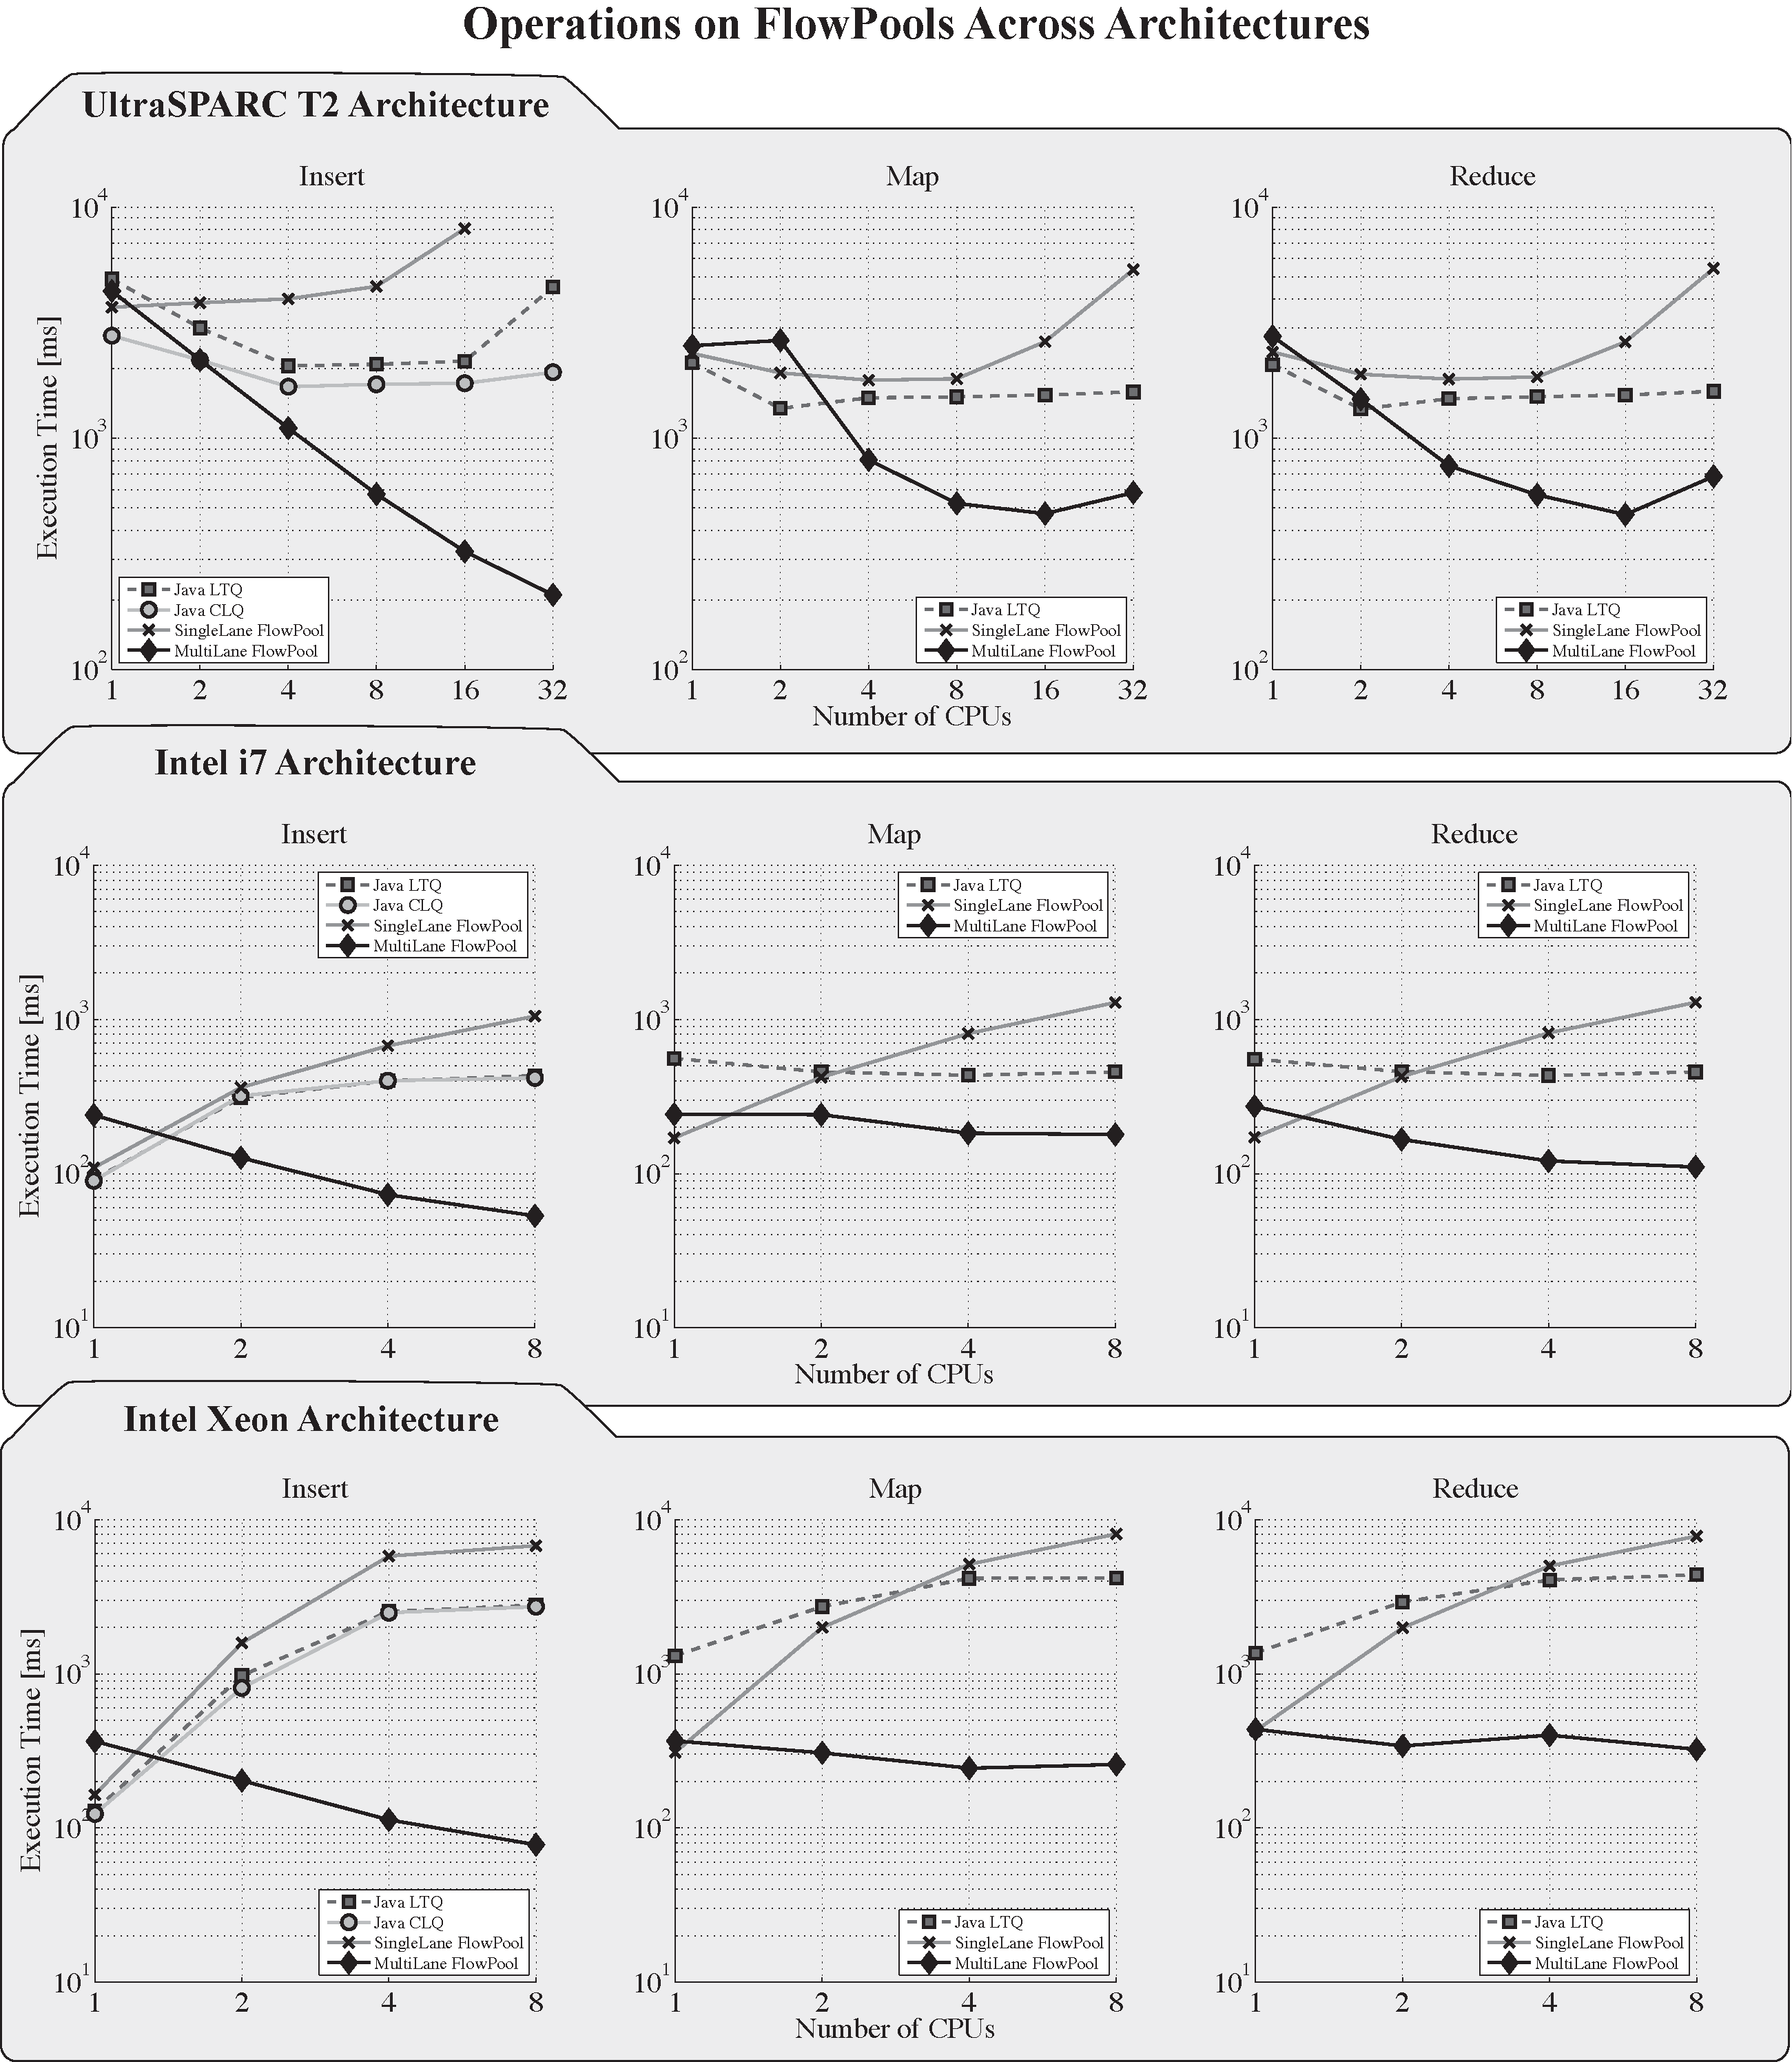
\includegraphics[width=\textwidth]{images/scaling-operations}
% 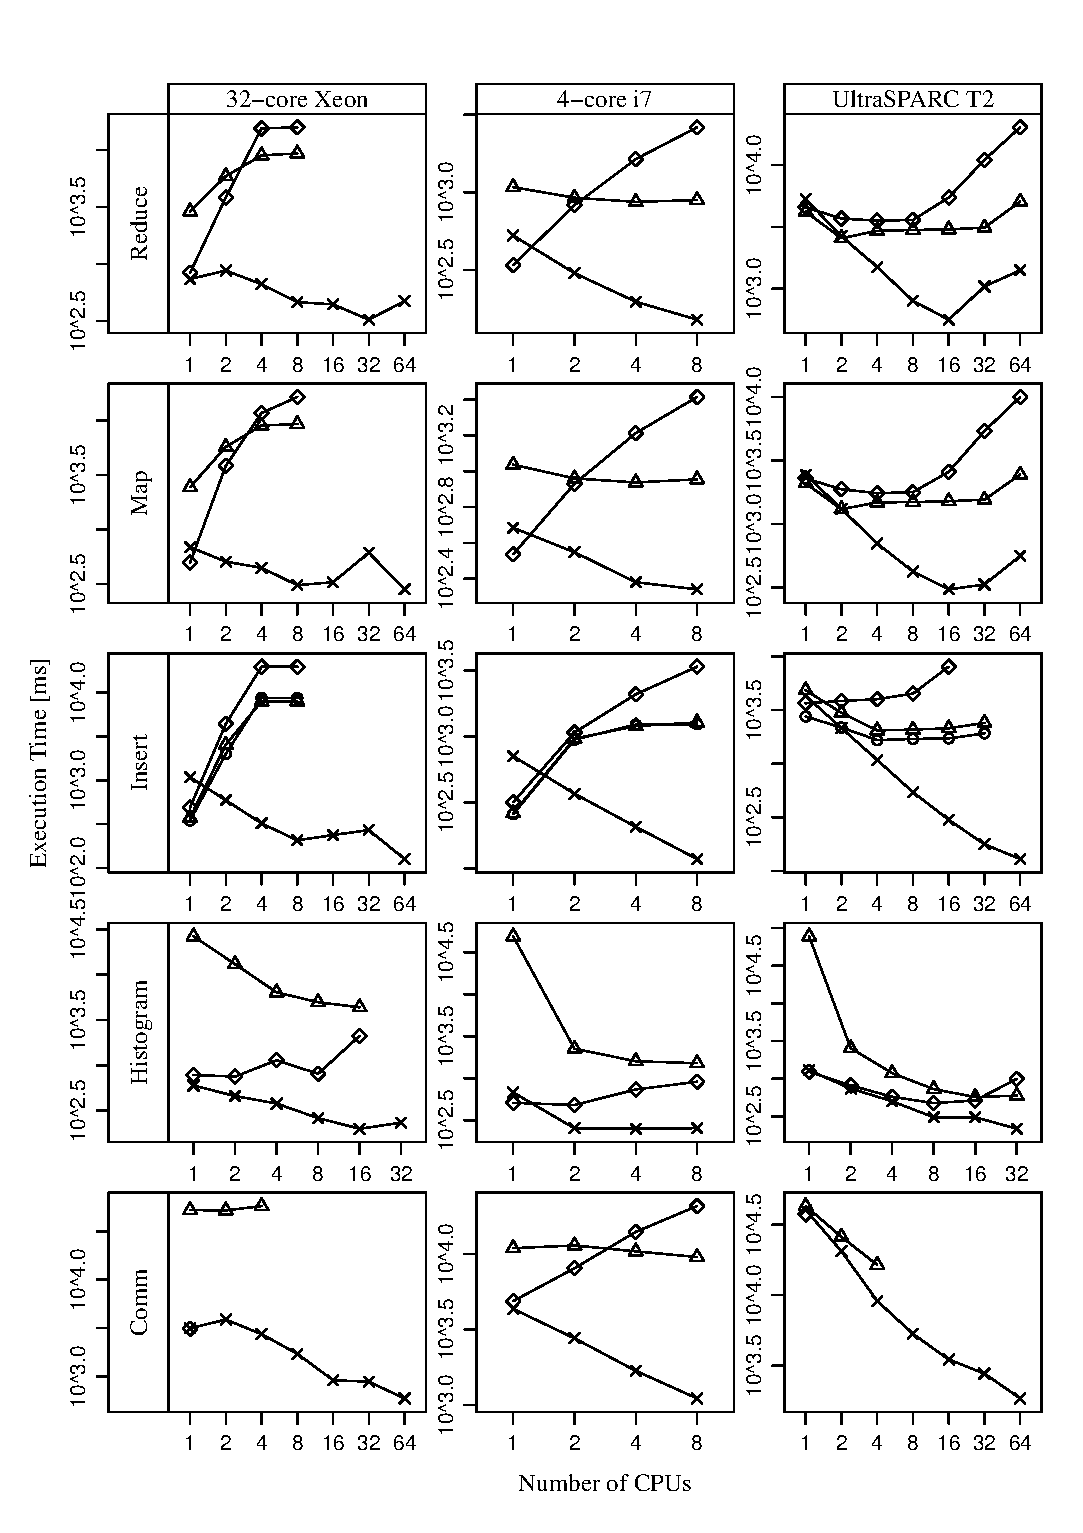
\includegraphics[width=\textwidth]{images/cpu-scaling}
\setlength{\abovecaptionskip}{-10pt}
\setlength{\belowcaptionskip}{-20pt}
\caption{Execution time vs parallelization across three different
architectures on three important FlowPool operations; insert, map,
reduce.}
\label{fig:eval-cpu-scaling}
%   $\Diamond$ single-lane FlowPool,
%   $\times$ multi-lane FlowPool,
%   $\triangle$ linked transfer queue,
%   $\circ$ concurrent linked queue} \label{fig:eval-cpu-scaling}
\end{figure}

In the \emph{Insert} benchmark, Figure \ref{fig:eval-cpu-scaling},
we evaluate concurrent insert operations, by distributing the
work of inserting $N$ elements into the data structure concurrently
across $P$ threads.
In Figure \ref{fig:eval-cpu-scaling}, it's evident that both single-lane FlowPools and concurrent queues do
not scale well with the number of concurrent threads, particularly
on the i7 architecture. They quickly slow down, likely due to cache
line collisions and CAS failures.
On the other hand, multi-lane FlowPools scale well, as threads
write to different lanes, and hence different cache lines,
meanwhile also avoiding CAS failures. This appears to reduce execution
time for insertions up to $54\%$ on the i7, $63\%$ on the
Xeon and $92\%$ on the UltraSPARC.

The performance of higher-order functions is evaluated in the \emph{Reduce},
\emph{Map} (both in Figure \ref{fig:eval-cpu-scaling}) and \emph{Histogram}
benchmarks (Figure \ref{fig:eval-hist-comm}).  It's important to note that the
\emph{Histogram} benchmark serves as a ``real life'' example, which uses both
the \verb=map= and \verb=reduce= operations that are benchmarked in Figure
\ref{fig:eval-cpu-scaling}. Also note that in all of these benchmarks, the
time it takes to insert elements into the FlowPool is also measured, since the
FlowPool programming model allows one to insert elements concurrently with the
execution of higher-order functions.

In the \textit{Histogram} benchmark, Figure \ref{fig:eval-hist-comm}, $P$ threads produce a total of
$N$ elements, adding them to the FlowPool.
The \verb=aggregate= operation is then used to produce 10 different
histograms concurrently with a different number of bins.
Each separate histogram is constructed by its own thread (or up to
$P$, for multi-lane FlowPools).
A crucial difference between queues and FlowPools here, is that with
FlowPools, multiple histograms are produced
by invoking several \verb=aggregate= operations, while queues require
writing each element to several queues-- one for each histogram.
Without additional synchronization, reading a single queue is not an
option, since elements have to be removed from the queue eventually, and
it is not clear to each reader when to do this.
With FlowPools, elements are automatically garbage collected when no
longer needed.

Finally, to validate the last claim of garbage being automatically
collected, in the \textit{Communication/Garbage Collection} benchmark,
Figure \ref{fig:eval-hist-comm}, we create a pool in which a
large number of elements $N$ are added concurrently by $P$
threads. Each element is then processed by one of $P$ threads through
the use of the \verb=aggregate= operation.
We benchmark against linked transfer queues, where $P$ threads concurrently remove
elements from the queue and process it.
For each run, we vary the size of the $N$ and examine its impact on the execution time.
Especially in the cases of the Intel architectures, the multi-lane
FlowPools perform considerably better than the linked transfer queues.
As a matter of fact, the linked transfer queue on the Xeon benchmark ran out of
memory, and was unable to complete, while the multi-lane FlowPool scaled effortlessly
to 400 million elements, indicating that unneeded elements are properly garbage collected.

\begin{figure}[t!]
\centering
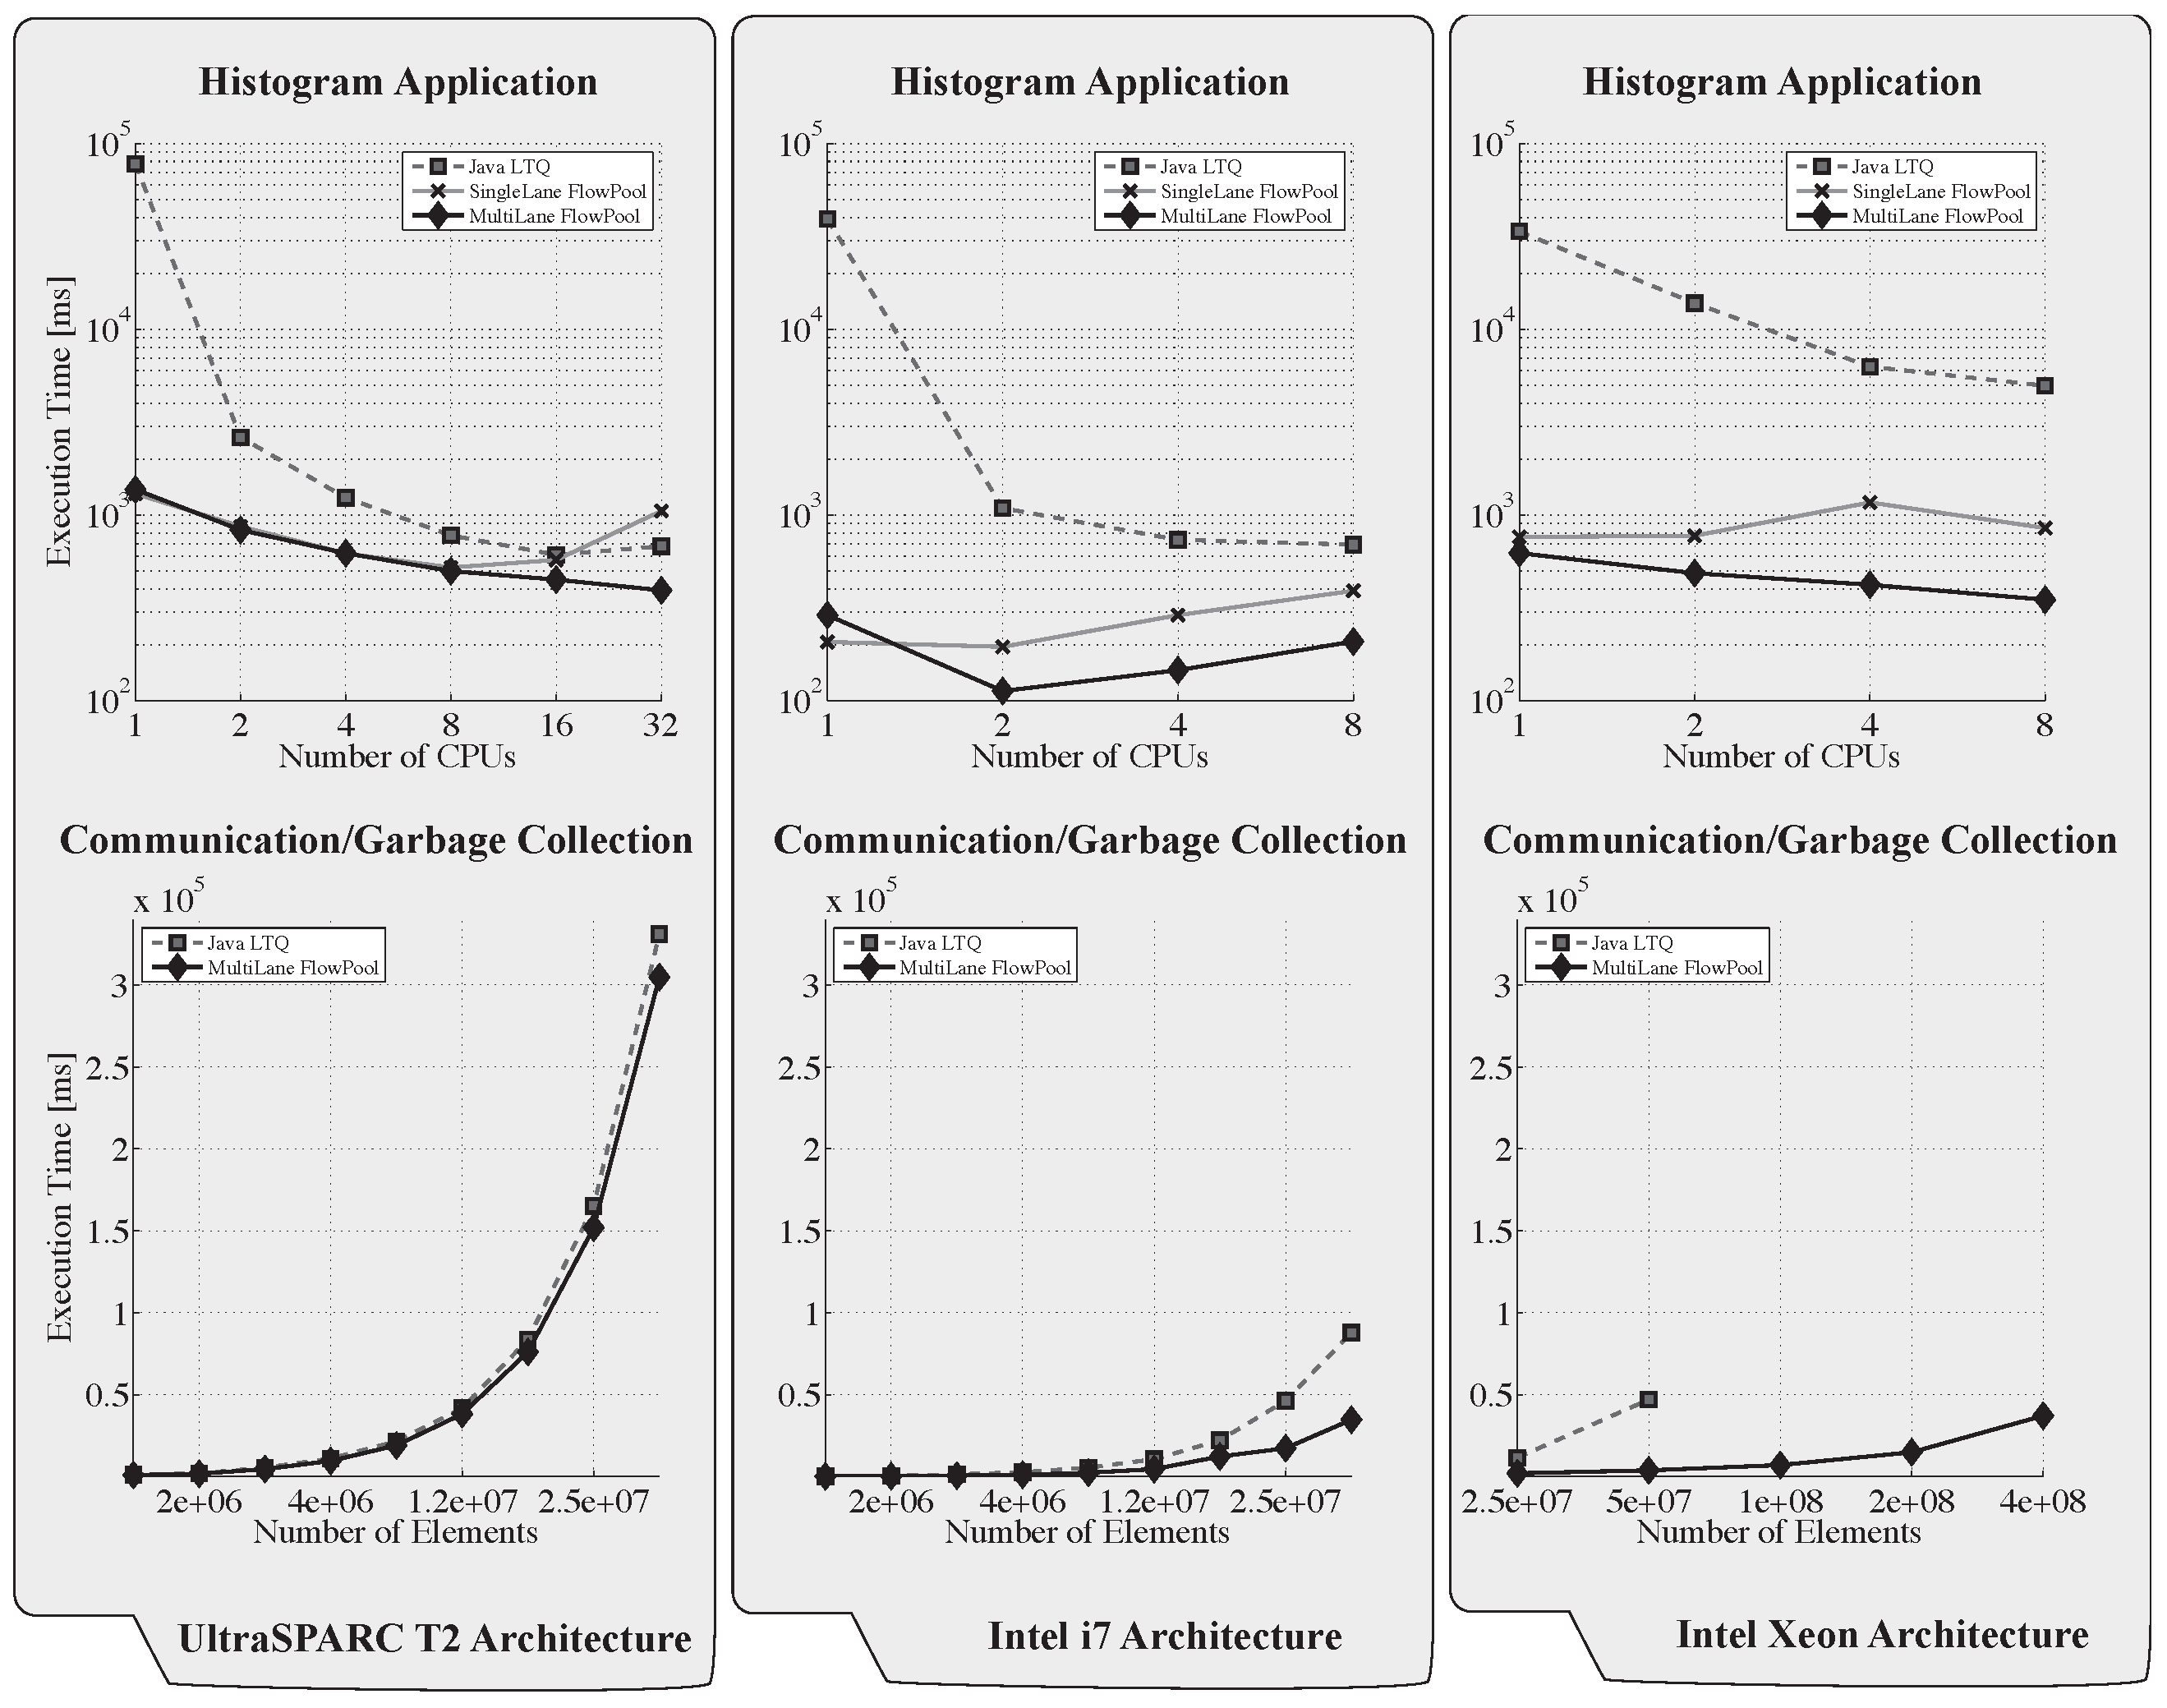
\includegraphics[width=\textwidth]{images/hist-comm}
\setlength{\abovecaptionskip}{-10pt}
\setlength{\belowcaptionskip}{-15pt}
\caption{Execution time vs parallelization on a real histogram application
(top), \& communication benchmark (bottom) showing memory efficiency,
across all architectures.}
\label{fig:eval-hist-comm}
%   $\Diamond$ single-lane FlowPool,
%   $\times$ multi-lane FlowPool,
%   $\triangle$ linked transfer queue,
%   $\circ$ concurrent linked queue} \label{fig:eval-cpu-scaling}
\end{figure}


\subsection{Related Work}

An introduction to linearizability and lock-freedom
is given by Herlihy and Shavit \cite{Herlihy08}.
A detailed overview of concurrent data structures is given
by Moir and Shavit \cite{Moir05}.
To date, concurrent data structures remain an active area of
research-- we restrict this summary to those relevant to this work.

Concurrently accessible queues have been present for a while,
an implementation is described by \cite{Mellor87}.
Non-blocking concurrent linked queues are described by Michael and
Scott \cite{Michael96}. This CAS-based
queue implementation is cited and used widely today, a variant of
which is present in the Java standard library.
More recently, Scherer, Lea and Scott \cite{SchererLS09} describe
synchronous queues which internally hold both data and requests.
Both approaches above entail blocking (or spinning) at least on the
consumer's part when the queue is empty.

While the abstractions above fit well in the concurrent imperative
model, they have the disadvantage that the programs written using them
are inherently nondeterministic.
Roy and Haridi~\cite{RoyH2004} describe the Oz programming language,
a subset of which yields programs deterministic by construction.
Oz dataflow streams are built on top of
single-assignment variables and are deterministically ordered.
They allow multiple consumers, but only one producer
at a time.
Oz has its own runtime which implements blocking using
continuations.
%Blocking is less efficient on the JVM, CLR and many native
%environments.

The concept of single-assignment variables is used to provide logical
variables in concurrent logic programming languages~\cite{Shapiro89}.
It is also embodied in
futures proposed by Baker and Hewitt \cite{Hewitt77}, and promises
first mentioned by Friedman and Wise \cite{Wise76}.
Futures were first implemented in MultiLISP \cite{Halstead85},
and have been employed in many languages and frameworks since.
Scala 2.10 futures~\cite{SIP14} and Twitter futures~\cite{TwitterFutures} are
of interest, because they define monadic operators and a
number of high-level combinators that create new futures.
These APIs avoid blocking.
Futures have been generalized to data-driven futures,
which provide additional information to the scheduler~\cite{Tasirlar11}.
Many frameworks have constructs that start an asynchronous
computation and yield a future holding its result, for example, Habanero Java~\cite{Shirako11} (\verb=async=)
and Scala~\cite{Odersky10} (\verb=future=).

A number of other models and frameworks recognized the need to embed
the concept of futures into other data-structures.
Single-assignment variables have been generalized to I-Structures~\cite{Arvind89} which are essentially
single-assignment arrays.
CnC~\cite{Burke11,CnC10} is a parallel programming model
influenced by dynamic dataflow, stream-processing and tuple spaces \cite{Gelernter85}.
In CnC the user provides high-level operations along with the ordering
constraints that form a computation dependency graph.
FlumeJava~\cite{Chambers10} is a distributed programming model which
relies heavily on the concept of collections containing futures.
An issue that often arises with dataflow programming models are
unbalanced loads.
This is often solved using bounded buffers which prevent
the producer from overflowing the consumer.
%Analytical approaches to modeling pipelined applications have also
%been addressed~\cite{Cascaval09}.

Opposed to the correct-by-construction determinism described thus far,
a type-systematic approach can also ensure that concurrent executions
have deterministic results.
Recently, work on Deterministic Parallel Java showed that a
region-based type system can ensure determinism~\cite{Bocchino09}.
X10's constrained-based dependent types can similarly ensure
determinism and deadlock-freedom~\cite{Saraswat07}.


\section{Conclusion}

% We have presented an abstraction and underlying data structure for
% deterministic concurrent dataflow programming. We achieve composability
% through the use of functional programming abstractions and non-blocking
% algorithms. We prove that our implementation is linearizable, lock-free, and
% deterministic. And finally, experimental results show that in many practical
% cases, FlowPools outperform comparable concurrent queue data structures
% present in the Java standard library.

% We have shown that deterministic higher-order operators can be built
% on top of \verb=<<= and \verb=foreach=, which corresponds to
% sequential collections.
% The prerequisite is that \verb=<<= can be invoked concurrently and
% that \verb=foreach= executes asynchronously.

% We emphasize a property of FlowPools which goes beyond
% a dataflow model such as Oz (or some other future/promise based
% model) in which more complex data structures such as streams are built
% on top of single-assignment variables.
% With single-assignment pools multiple threads can add elements without
% agreeing on where the added element should structurally be, as is the
% case with dataflow streams.
% A consequence of this is a more flexible programming model.

The abstraction for concurrent dataflow programming we
presented provides a composable deterministic programming model.
It can be implemented in a provably non-blocking manner
and is efficient as well, as shown in experiments.

As future work, we plan developing other
concurrent collection types with deterministic semantics, which enrich
the correct-by-construction single-assignment model, such as
bounded buffers, streams and maps.
On the implementation level, we anticipate the need of embedding the
callbacks within the data-structure itself, as is the case with
callback-based futures and FlowPools -- this has a particular
benefit on platforms which do not support efficient
continuations.
